% PBGIA interdisciplinary manuscript -- focused revision, 17 November 2026.
% Journal-neutral article format, NOT a publisher-specific submission template.
% Replace author information and declarations after coauthor approval.
% Figures 3 and 7 use computed N=30 spin fields; real-image director pilots are distinguished from synthetic tests.
\documentclass[11pt,a4paper]{article}
\usepackage[margin=1in]{geometry}
\usepackage[T1]{fontenc}
\usepackage[utf8]{inputenc}
\usepackage{lmodern}
\usepackage{amsmath,amssymb,amsfonts,bm,mathtools}
\usepackage{booktabs,tabularx,threeparttable,multirow,array}
\usepackage{graphicx,float,placeins}
\usepackage{caption,subcaption}
\usepackage[numbers,sort&compress]{natbib}
\usepackage{microtype}
\usepackage{xurl}
\usepackage{siunitx}
\usepackage{xcolor}
\usepackage[colorlinks=true,linkcolor=blue!50!black,citecolor=blue!50!black,urlcolor=blue!50!black]{hyperref}
\usepackage{enumitem}
\captionsetup{font=small,labelfont=bf}
\setlength{\parskip}{0.25em}
\setlength{\parindent}{1.2em}
\newcommand{\nn}{\bm n}
\newcommand{\vv}{\bm v}
\newcommand{\xx}{\bm x}
\newcommand{\dd}{\mathrm{d}}
\newcommand{\bbZ}{\mathbb Z}
\newcommand{\RP}{\mathbb{RP}}
\newcommand{\Sn}{\mathbb S}
\newcommand{\gt}{\mathrm{GT}}
\newcommand{\rel}{\mathrm{rel}}
\newcommand{\energy}{\mathcal E}
\newcommand{\Ham}{\mathcal H}
\newcommand{\degree}{\operatorname{deg}}
\newcommand{\Tr}{\operatorname{tr}}
\newcommand{\MARE}{\mathrm{MARE}}
\newcommand{\diff}{\partial}
\newcommand{\figurepath}[1]{figures/#1.pdf}
\newcommand{\journote}[1]{{\sloppy\textcolor{red!65!black}{[EDITORIAL NOTE: #1]}\par}}
\title{Binary-field-driven spin textures as an analyzable, scale-selective representation of image geometry, orientation and topology}
\author{Author list and affiliations to be confirmed by the research team}
\date{Revised draft --- 17 November 2026}

\begin{document}
\maketitle

\begin{abstract}
Can the geometry of an image be read from the magnetization it would induce? We treat a binary image as a static field $f=\pm1$ acting on a unit-vector spin and let a simple alignment rule generate the response. Boundaries then become domain walls, the transverse spin in each wall points along the boundary normal, and the topology of the image is carried by the integer degree of the spin map. The rule is not a gradient flow of any energy, so we develop its theory directly from its fixed points. The resulting picture is unexpectedly complete. A planar wall obeys a pendulum-like equation in which the chiral coupling acts as a nonconservative force, and its width collapses onto a single scaling function of $\kappa=D/\sqrt{Jh}$. On the lattice, an exact sign rule turns the generated field into a scale-selective filter that removes isolated defects. The coarea formula, together with lattice symmetry, converts the total variation of the field into a perimeter or area estimate that needs no reference shape. Averaging the transverse spin projectively yields an $\RP^1$ director field whose half-integer defects obey exact scale-space laws: conservation across Gaussian windows, a Bessel-function core, pair annihilation at $\sigma_c=0.441\,d$, and a parameter-free density $1/4\pi\sigma^2$ for orientationally random textures. The spin degree, in turn, equals the Euler characteristic of the generated domain by Hopf's theorem. Each prediction is confirmed numerically. On a benchmark of 294 shapes with exact perimeters and areas, the readout without any calibration is more accurate than every calibrated conventional estimator in 2D (0.54\% versus 0.70--1.17\%), equals calibrated marching cubes in 3D (0.35\%), and remains the most accurate under salt-and-pepper noise. Its residual error follows a quantization law and lies within a factor 1.3--3.3 of an information bound for disks. On an experimental Lorentz image of a skyrmion lattice, the degree per skyrmion is $1.0000\pm0.0015$ over 1074 skyrmions. The physics of the generated texture thus explains both when the method works and where it must fail.
\end{abstract}

\noindent\textbf{Keywords:} binary images; domain walls; nonvariational dynamics; coarea formula; lattice metrication; scale-selective filtering; nematic defects; topological degree.


\section*{Introduction}
A ferromagnet placed in a nonuniform field reveals the shape of that field. Where the field reverses, the magnetization must turn, and the turning region---a domain wall---follows the contour of the reversal. The wall carries more than position: its transverse magnetization points across the contour, its energy grows with the contour's length, and the way the magnetization wraps the sphere of directions counts the enclosed domains. This paper asks whether the converse is useful. If a binary image is read as such a field, does the magnetization it induces provide a principled, analyzable representation of the image's geometry?

The question matters because image geometry is usually obtained piece by piece. Lengths come from contour tracing or Crofton counting, areas from marching cubes \cite{Lorensen1987}, orientations from structure tensors \cite{Bigun1991}, and connectivity from Euler analysis. Each tool is efficient, but each starts again from the raw raster, and their accuracies, failure modes and parameter dependences are not connected by any common principle. A field theory of the image would supply such a principle, provided its behavior can be derived rather than tuned.

Our group has used fragments of this idea before. Skyrmion-like charges count objects \cite{Park2024AMT}, an $(N+1)$-component chiral field computes Euler characteristics of $N$-dimensional objects \cite{Moon2025SR}, and a magnetic structure tensor analyzes defects in fingerprints \cite{Park2025iScience}. Diffuse-interface measures of boundary extent \cite{Modica1987,Allen1979,Chan2001} and total-variation functionals \cite{Rudin1992} rest on related intuitions. In all of these, however, the magnetic picture served as motivation. The algorithms that are actually run---fast, synchronous alignment updates---do not minimize the energy that inspired them, so energy arguments cannot say how wide the walls are, how accurate a measurement will be, or when the generated field departs from the input.

Here we close this gap by treating the alignment rule itself as the physical system. We show that, although it admits no energy function, its fixed points obey closed equations, and that each geometric readout is governed by an identifiable mechanism. Wall widths follow a scaling law in which the chiral coupling enters as a nonconservative force. On the lattice, an exact sign rule makes the field a filter with a sharp size threshold. The coarea formula and lattice symmetry turn the field's total variation into a reference-free measure of boundary extent. A projective average of the transverse spin yields a director field whose half-integer defects obey exact laws under a change of observation scale. Finally, Hopf's theorem identifies the spin degree with the Euler characteristic of the generated domain. We then test each prediction numerically, including on a benchmark of shapes with exact perimeters and areas that spans convex, non-convex and near-contact geometries. Where the method fails, the same theory says why.

The paper is organized as follows. Section~\ref{sec:model} introduces the rule and its exact symmetries. Section~\ref{sec:theory} develops the theory of walls, filtering, boundary measurement, director defects and the degree. Section~\ref{sec:results} confronts these predictions with computation, and Sec.~\ref{sec:discussion} discusses where the model's assumptions agree with what is observed and why.

\section{Model and exact symmetries}\label{sec:model}
\subsection{Binary source, spin field and update rule}
Let $\Lambda\subset a\mathbb Z^d$ ($d=2,3$) be a pixel or voxel lattice with spacing $a$. A binary mask defines the fixed source
\begin{equation}
 f_i=\begin{cases}+1,& i\text{ inside the object},\\ -1,& i\text{ outside}.\end{cases}
 \label{eq:binary}
\end{equation}
At every site we place a $(d+1)$-component unit vector
\begin{equation}
 \nn_i=(\vv_i,s_i)\in\Sn^d,\qquad \vv_i\in\mathbb R^d,\quad |\vv_i|^2+s_i^2=1 .
 \label{eq:spin}
\end{equation}
A two-dimensional image is thus represented by an $\Sn^2$-valued field and a volume by an $\Sn^3$-valued field. The scalar component $s$ follows the source away from boundaries; the transverse vector $\vv$ is appreciable only inside walls. The field is initialized from the Euclidean distance transform of the rasterized mask: $s^{(0)}=\tanh(\xi/2.3)$ with $\xi$ the signed distance, and $\vv^{(0)}$ along the discrete gradient of $s^{(0)}$ with length $\sqrt{1-s^2}$. No analytic shape information enters the generator.

The field is then updated synchronously for a fixed number of steps $N$,
\begin{align}
 \bm H_{v,i}&=J\!\!\sum_{j\in\mathrm{NN}(i)}\!\!\vv_j+D\,(Gs)_i,\label{eq:updatev}\\
 H_{s,i}&=J\!\!\sum_{j\in\mathrm{NN}(i)}\!\! s_j+h f_i,\label{eq:updates}\\
 \nn_i&\leftarrow\bm H_i/|\bm H_i|\quad(|\bm H_i|>10^{-12};\ \text{otherwise unchanged}),\label{eq:updaten}
\end{align}
where $\mathrm{NN}(i)$ are the $2d$ axial neighbors and $G$ is the centered difference, $(Gs)_i=\{(s_{i+\hat e_\alpha}-s_{i-\hat e_\alpha})/2\}_{\alpha=1}^d$. The main setting is $J=D=1$, $h=2$ and $N=30$, on periodic arrays padded so that objects stay away from the edges. Figure~\ref{fig:concept} shows the resulting field and readout for one shape.

\begin{figure}[t]
\centering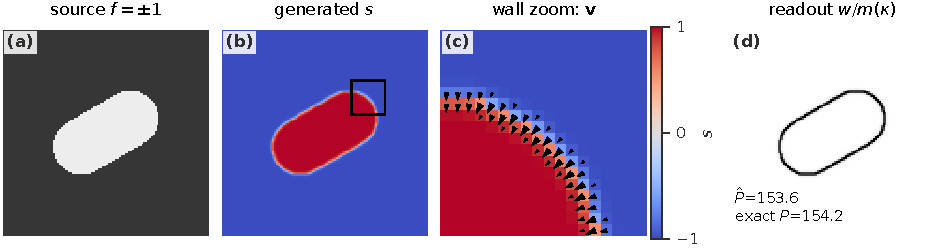
\includegraphics[width=\linewidth]{figures/Fig1_concept.pdf}
\caption{\textbf{A fixed binary source generates a smooth spin texture whose wall carries every geometric readout.} (a) Source $f=\pm1$ for a rotated stadium ($R=15$, $L=30$). (b) Scalar component $s$ after $N=30$ updates of Eqs.~\eqref{eq:updatev}--\eqref{eq:updaten}; the box marks the region enlarged in (c). (c) Transverse component $\vv$ (arrows) on the wall, pointing along the inward normal. (d) Local readout density of Eq.~\eqref{eq:refree}; its sum gives the perimeter without any reference shape. Colors of $s$ share the bar shown; $J=D=1$, $h=2$.}
\label{fig:concept}
\end{figure}

\subsection{The update is not a gradient flow}\label{subsec:nonvar}
The effective field is affine in the spins, $\bm H=W\nn+\bm b$ with $\bm b=(0,hf)$. A field of this form is the negative gradient of an energy, $\bm H=-\nabla_{\nn}E$, if and only if $W$ is symmetric. In that case $E=-\tfrac12\nn^{\mathsf T}W\nn-\bm b^{\mathsf T}\nn$ up to a constant, because an affine gradient field has a quadratic potential. In Eqs.~\eqref{eq:updatev}--\eqref{eq:updates}, the block coupling $s$ into $\bm H_v$ is $DG$, while the block coupling $\vv$ into $H_s$ vanishes. Hence $W$ is not symmetric for $D\neq0$, and \emph{no energy function exists whose constrained steepest-alignment dynamics is Eq.~\eqref{eq:updaten}}.

It is useful to split the chiral coupling into a reciprocal and a nonreciprocal half,
\begin{equation}
 \begin{pmatrix}\bm H_v\\ H_s\end{pmatrix}\ni
 \underbrace{\frac D2\begin{pmatrix}Gs\\ -G^{\!*}\!\cdot\vv\end{pmatrix}}_{\text{reciprocal}}
 +\underbrace{\frac D2\begin{pmatrix}Gs\\ +G^{\!*}\!\cdot\vv\end{pmatrix}}_{\text{nonreciprocal}},
 \qquad G^*=-G\ \text{(periodic)}.
 \label{eq:split}
\end{equation}
The reciprocal half derives from the interfacial (N\'eel-type) Lifshitz invariant of a lattice Hamiltonian $\Ham=-J\sum_{\langle ij\rangle}\nn_i\!\cdot\!\nn_j-h\sum_if_is_i-\tfrac D2\sum_i\vv_i\!\cdot\!(Gs)_i$. The nonreciprocal half has no Hamiltonian counterpart. Energy-based arguments, such as wall tension or monotone energy decrease, therefore apply at most to the reciprocal part. Section~\ref{subsec:fixedpoint} shows that, for planar walls, the reciprocal part does not affect the profile at all.

\subsection{Exact symmetries}\label{subsec:symm}
Four exact properties constrain everything that follows.
\begin{enumerate}[label=(S\arabic*),leftmargin=2.4em,itemsep=0.1em]
\item \emph{Scale invariance.} Multiplying $(J,D,h)$ by any positive constant leaves $\bm H/|\bm H|$ unchanged. Only $h/J$ and $D/J$ matter.
\item \emph{Lattice covariance.} The update commutes with the point group of the lattice ($C_{4v}$ in 2D, $O_h$ in 3D), with $\vv$ transforming as a polar vector. We verified this numerically to $1.2\times10^{-7}$ under axis permutations in float32.
\item \emph{Inside--outside symmetry.} $(f,s,\vv)\to(-f,-s,-\vv)$ maps solutions to solutions. Objects and holes of the same shape are therefore treated identically; we confirmed this for all test features in Fig.~\ref{fig:filter}(a).
\item \emph{Chirality symmetry.} $(D,\vv)\to(-D,-\vv)$ at fixed $(f,s)$ maps solutions to solutions, because $H_s$ does not contain $\vv$. The scalar field, and every readout built from it, depends on $D$ only through the product $cD$, where $c=\pm1$ is the wall chirality (the sign of $\vv\cdot\nabla s$). The distance-transform initialization fixes $c=+1$.
\end{enumerate}
(S4) follows directly from the nonreciprocity in Eq.~\eqref{eq:split}. A reciprocal model would instead couple the sign of $D$ to the energy of each chirality.

\section{Theory of the generated texture}\label{sec:theory}
\subsection{Fixed points: walls with a nonconservative chiral force}\label{subsec:fixedpoint}
A fixed point of Eq.~\eqref{eq:updaten} requires $\nn_i\parallel\bm H_i$ with $\nn_i\cdot\bm H_i>0$. Equivalently, the component of $\bm H_i$ perpendicular to $\nn_i$ must vanish. In the continuum limit, $\sum_{\rm NN}\nn_j=2d\,\nn+a^2\nabla^2\nn+O(a^4\nabla^4)$. The term $2dJ\nn$ is parallel to $\nn$ and drops out of the condition. For a planar wall with normal coordinate $u$, $f=\operatorname{sgn}u$, and $\nn=(c\sin\theta\,\bm\nu,\cos\theta)$, we project onto $\bm e_\theta=(c\cos\theta\,\bm\nu,-\sin\theta)$. Using $\partial_u^2\nn\cdot\bm e_\theta=\theta''$ gives
\begin{equation}
 \boxed{\;Ja^2\,\theta''=h f\sin\theta+cD\,\sin\theta\cos\theta\,\theta'\;}
 \label{eq:fixedODE}
\end{equation}
In the reference energy model the chiral term integrates to a constant across a planar wall and leaves the profile untouched. Here it survives as a force proportional to $\theta'$. The corresponding mechanical quantity $\mathcal E=\tfrac12Ja^2\theta'^2-h(1-f\cos\theta)$ is not conserved:
\begin{equation}
 \frac{\dd\mathcal E}{\dd u}=cD\sin\theta\cos\theta\,(\theta')^2 .
\end{equation}
The force is damping on one side of the wall center and anti-damping on the other. Under the reflection $u\to-u$, $\theta\to\pi-\theta$ it is odd, so the wall stays centered on the input boundary while its width changes. Writing $t=u/\ell$, the equation becomes
\begin{equation}
 \theta_{tt}=f\sin\theta+\kappa\sin\theta\cos\theta\,\theta_t,\qquad
 \ell=a\sqrt{J/h},\qquad \kappa=\frac{cD}{\sqrt{Jh}} .
 \label{eq:scaled}
\end{equation}
Equation~\eqref{eq:scaled} contains no other parameter. Any width measure therefore obeys the exact scaling law
\begin{equation}
 w=\ell\,F(\kappa).
 \label{eq:collapse}
\end{equation}
For $\kappa=0$ the symmetric solution is the classical profile $\theta=4\tan^{-1}(qe^{-u/\ell})$ for $u\ge0$, with $q=\sqrt2-1$ and $\theta(-u)=\pi-\theta(u)$. For $\kappa\neq0$, write $Q(\theta)=|\theta_t|$ on $u>0$. Then $QQ_\theta=\sin\theta-\kappa\sin\theta\cos\theta\,Q$ with $Q(0)=0$. Expanding about $Q_0=2\sin(\theta/2)$ gives the center slope
\begin{equation}
 |\theta'(0)|=\frac{\sqrt2}{\ell}\bigl[1-K\kappa+O(\kappa^2)\bigr],\qquad
 K=\int_0^{\pi/2}\!\sin\phi\cos\phi\sin\tfrac{\phi}{2}\,\dd\phi=\frac{2\sqrt2}{15}.
 \label{eq:slope}
\end{equation}
Positive $\kappa$ widens the wall. The analytic profile is the one usually quoted for the reference energy model. It is now a property of the actual algorithm, but only at $\kappa=0$ and only for $\ell\gg a$.

\emph{Two regimes.} The continuum description requires $\ell\gg a$, that is $h/J\ll1$. The main setting $h/J=2$ gives $\ell=0.71a$: the walls are lattice-scale objects. This regime is chosen deliberately. It pins the scalar zero level to the raster boundary, so clean masks are reproduced with Dice $=1$ for all 2D test shapes down to disks of radius $1.5$ pixels, and for 3D shapes of radius $\ge6$ voxels (a radius-2 sphere loses 13\% of its voxels). It also activates the discrete filtering rule of Sec.~\ref{subsec:stability}. In this regime Eq.~\eqref{eq:collapse} is only qualitative, and the wall width must be measured (Fig.~\ref{fig:wallth}).

\subsection{Lattice regime: a local stability law and scale selectivity}\label{subsec:stability}
Because $s_i\leftarrow H_{s,i}/|\bm H_i|$, the \emph{sign} of $s_i$ after one update equals the sign of $H_{s,i}$ exactly. $H_{s,i}$ contains neither $D$ nor $\vv$. Consider a site whose input sign is $\sigma_i=f_i$, with $z_{\rm in}$ neighbors of the same sign and $z_{\rm out}=2d-z_{\rm in}$ of opposite sign. In the Ising limit $|s_j|\simeq1$, the site keeps its sign if and only if
\begin{equation}
 \boxed{\;h>J\,(z_{\rm out}-z_{\rm in})\;}
 \label{eq:stability}
\end{equation}
Equation~\eqref{eq:stability} has four immediate consequences.
\begin{enumerate}[label=(\roman*),leftmargin=2em,itemsep=0.1em]
\item An isolated pixel or voxel survives only if $h>2dJ$. In the main setting ($h=2J$), salt-and-pepper defects are removed in both 2D and 3D. This is the mechanism behind the noise robustness reported below, and it acts in the first update.
\item Sites with too few like neighbors erode. In 2D with $h=2J$, sites with one like neighbor are marginal: domino- and line-end sites. In 3D with $h=2J$, sites with two or fewer like neighbors are unstable, so one-voxel-thick sheets, edges and necks erode.
\item The sign dynamics is independent of $D$ up to the neighbors' $|s_j|<1$ corrections. Hence $h/J$ sets the filtering scale while $\kappa$ sets the wall width (Sec.~\ref{subsec:fixedpoint}). The two can be tuned separately.
\item The same rule that removes noise removes true features below the threshold, and it can change topology (Sec.~\ref{subsec:topo}).
\end{enumerate}
The rule neglects the reduction of $|s_j|$ near walls. It is therefore exact for decisions far from marginal and approximate near equality, and it breaks down when $\ell\gtrsim a$ (small $h$). There, curvature-driven shrinkage of objects a few $\ell$ across takes over.

\subsection{Boundary readout: coarea identity, Steiner corrections and lattice metrication}\label{subsec:readout}
We read boundary extent from half the total variation of the scalar component,
\begin{equation}
 I_{\rm TV}=\frac12\int_\Omega|\nabla s|\,\dd^dx .
\end{equation}
By the coarea formula,
\begin{equation}
 I_{\rm TV}=\frac12\int_{-1}^{1}\mathcal A_{d-1}\bigl(\partial\{s>t\}\bigr)\,\dd t ,
 \label{eq:coarea}
\end{equation}
which holds exactly for any Lipschitz $s$. $I_{\rm TV}$ is therefore the perimeter (2D) or surface area (3D) of the level sets of $s$, averaged uniformly over $t\in(-1,1)$. No wall-width calibration is required, provided each level set is present, i.e.\ the field saturates to $\pm1$ on both sides. Thin features that never saturate are underestimated. For a disk, Eq.~\eqref{eq:coarea} reduces to $I_{\rm TV}=2\pi\langle r\rangle_w$, with weight $w=\tfrac12|\partial_rs|$.

If the level set at height $t$ is the parallel set of the true boundary at normal offset $u(t)$, Steiner's formula gives
\begin{equation}
 I_{\rm TV}^{(2D)}=P+2\pi\chi\langle u\rangle,\qquad
 I_{\rm TV}^{(3D)}=S+2M\langle u\rangle+2\pi\chi\langle u^2\rangle,
 \label{eq:steiner}
\end{equation}
where $M=\int H\,\dd S$ is the integrated mean curvature, $\chi$ the Euler characteristic, and $\langle\cdot\rangle$ the average over $t$. In 2D the curvature bias is purely topological and vanishes for walls centered on the boundary. Section~\ref{subsec:fixedpoint} predicts such centering, and it is observed: $|\langle u\rangle|<0.021$ pixels for disks with $R\ge8$.

On the lattice, the remaining error is \emph{metrication}: the discrete $|\nabla s|$ of a planar wall depends on its orientation. Let $m(\bm\nu)$ be $I_{\rm TV}$ per unit area of an infinite planar wall with normal $\bm\nu$, computed with the same generator. Three exact statements follow.
\begin{enumerate}[label=(\alph*),leftmargin=2em,itemsep=0.1em]
\item By (S2), $m$ is invariant under the lattice point group. In 2D it is a Fourier series in $\cos4k\varphi$ only.
\item $m=1$ exactly along the lattice directions [10] and [11] in 2D, and [100], [110] and [111] in 3D. For these directions the profile depends on one lattice coordinate, so the centered differences telescope: the sum of $|Gs|$ across the wall equals the total rise $2$.
\item For a surface whose normals are distributed uniformly, the readout is multiplied by the orientation average $\bar m_d$.
\end{enumerate}
For the main setting, $\bar m_2=1.0189$ and $\bar m_3=1.0160$ (Sec.~\ref{subsec:res:metric}). The chiral coupling reduces metrication: at $D=0$, $\bar m_2=1.0437$, because the wider walls of Eq.~\eqref{eq:slope} are sampled more smoothly.

\emph{Curvature-dependent metrication.} Walls of width $\sim a$ do not resolve curvature radii of a few lattice spacings, so the factor relating $I_{\rm TV}$ to the true extent also depends on local curvature. By symmetry this dependence enters through rotation-invariant curvature scalars. We use the mean curvature, $\kappa$ in 2D and $2H$ in 3D, and write
\begin{equation}
 m_d(\kappa)=\bar m_d+b_1|a\kappa|+b_2(a\kappa)^2+b_3|a\kappa|^3 .
 \label{eq:mkappa}
\end{equation}
The coefficients are fitted once to disks and spheres with radii $2.5$--$40$ lattice spacings (Fig.~\ref{fig:metric}). The constant term is fixed by the planar walls, not fitted. The field itself supplies the local curvature, $\kappa=-\nabla\cdot(\nabla\tilde s/|\nabla\tilde s|)$, where $\tilde s$ is $s$ smoothed with a unit Gaussian. On disks and spheres, its wall-weighted mean agrees with $1/R$ and $2/R$ to within a few percent. The resulting \emph{reference-free} estimator is
\begin{equation}
 \widehat{\mathcal A}_{d-1}=\sum_x\frac{\tfrac12|Gs|_x}{m_d(\kappa_x)} ,
 \label{eq:refree}
\end{equation}
which reduces to $I_{\rm TV}/\bar m_d$ for flat boundaries. No benchmark shape, and no shape of the evaluation set, enters its constants.

\emph{Direction-resolved metrication.} The orientation average $\bar m_d$ is exact only for boundaries whose normals are uniformly distributed. A straight edge at angle $\varphi$ is measured with the factor $m(\varphi)$ instead, and Fig.~\ref{fig:metric}(a) shows that $m$ varies by up to 3\% between $0^\circ$ and $45^\circ$. Because the stencil and the generator are covariant under $C_{4v}$, $m(\varphi)$ is even and has period $\pi/2$, so it expands in the invariant harmonics only:
\begin{equation}
 m(\varphi,\kappa)=c_0+\sum_{j=1}^{6}c_j\cos4j\varphi+\Delta(\kappa),\qquad \Delta(\kappa)=b_1|a\kappa|+b_2(a\kappa)^2+b_3|a\kappa|^3 .
 \label{eq:mphikappa}
\end{equation}
The coefficients $c_j$ follow from planar walls at 46 rational orientations, and $\Delta$ is fitted to the residual of disks after the direction correction. The local normal angle $\varphi$ is read from the same smoothed field as $\kappa$. Replacing $m_d(\kappa)$ by Eq.~\eqref{eq:mphikappa} in Eq.~\eqref{eq:refree} removes the systematic error of straight boundaries at unfavorable angles. In 3D the analogous expansion in cubic harmonics did not improve the readout, because the planar factor is a less smooth function on $\Sn^2$ (fit residual $1.2\%$ against $0.45\%$ in 2D). We therefore use the orientation-averaged law in 3D. A transversally smoothed difference stencil, $[\alpha,1-2\alpha,\alpha]\otimes\tfrac12[-1,0,1]$, offers an alternative route to isotropy. It halves the spread of $m(\varphi)$ at $\alpha=1/4$, but it also broadens the response near contacts, and the explicit correction performed better.

\emph{Predicted failure: merging level sets.} Equation~\eqref{eq:coarea} counts every level set once. If two objects are separated by a gap narrower than the wall, the level sets $\{s>t\}$ for $t$ below the saddle value of $s$ in the gap join the two objects into one region. The facing parts of their boundaries then drop out of $\mathcal A_{d-1}(\partial\{s>t\})$, and the Steiner term in Eq.~\eqref{eq:steiner} switches from $\chi=2$ to $\chi=1$ for those levels. The readout is therefore biased low whenever the gap is comparable to the wall width.

The derivative-energy readout $I_E=\int\sum_a|\nabla n_a|^2$ used in earlier work depends on the wall profile through $\int\theta'^2\dd u$. It therefore requires calibration and inherits the $\kappa$ and curvature dependence of the width. We retain it only for comparison.

\subsection{Orientation tensors and the projective director}\label{subsec:orient}
\emph{Normals and global axes.} Along a resolved wall, $\vv$ points along the inward normal. The transverse tensor $\int\omega(s)\vv\vv^{\mathsf T}$ and the derivative Gram tensor $T_{ij}=\int\partial_i\nn\cdot\partial_j\nn$ measure the distribution of boundary normals. For an elongated body, the axis of \emph{least} normal weight is the long axis; for a long fiber, the minimum-eigenvalue axis is the fiber direction. Neither tensor encodes the separation of disconnected isotropic objects, which is carried by the spatial covariance $C_{ij}$ of a wall-localized weight. This distinction is information-theoretic rather than numerical: the local normal distribution of two circles does not depend on how they are placed.

\emph{Why the local orientation is projective.} In a striped or fibrous texture, neighboring walls bound domains of opposite sign, so their inward normals point in opposite directions. Fields generated at different intensity thresholds $t_k$ can also reverse the sign of $\vv$ at the same place. A coarse-grained \emph{vector} average of $\vv$ therefore cancels, while the outer product $\vv\vv^{\mathsf T}$, invariant under $\vv\to-\vv$, survives. We define the scale-$\sigma$ orientation tensor
\begin{equation}
 Q_\sigma(\bm x)=\frac1K\sum_{k=1}^{K}\int G_\sigma(\bm x-\bm y)\,\vv_k(\bm y)\vv_k(\bm y)^{\mathsf T}\,\dd^d y ,
 \qquad G_\sigma(\bm x)=\frac{e^{-|\bm x|^2/2\sigma^2}}{(2\pi\sigma^2)^{d/2}},
 \label{eq:Qsigma}
\end{equation}
where $\vv_k$ is the transverse field generated from the binary map at threshold $t_k$ ($K=1$ for a binary input). $Q_\sigma$ is symmetric and positive semidefinite. Where its largest eigenvalue is nondegenerate, the eigenline defines the normal director $[\bm d]\in\RP^{d-1}$; in 2D the tangent director is the orthogonal line.

In 2D it is convenient to encode the traceless part in one complex number,
\begin{equation}
 q_\sigma\equiv(Q_{xx}-Q_{yy})+2iQ_{xy}=|q_\sigma|\,e^{2i\varphi},\qquad
 \lambda_1-\lambda_2=|q_\sigma|,\qquad S_\sigma=\frac{|q_\sigma|}{\operatorname{tr}Q_\sigma}\in[0,1],
 \label{eq:qcomplex}
\end{equation}
where $\varphi$ is the angle of the normal director, defined modulo $\pi$, and $S_\sigma$ is the coherence. The factor $2$ in the phase is the algebraic form of projectivity: $\varphi$ and $\varphi+\pi$ give the same $q_\sigma$. Because Eq.~\eqref{eq:Qsigma} is a linear convolution,
\begin{equation}
 q_\sigma=G_\sigma*q_0 ,
 \label{eq:scalespace}
\end{equation}
with $q_0$ the unsmoothed, pixel-level field. The family $\{q_\sigma\}$ is thus a linear scale space of a complex field. The window $\sigma$ is the single parameter that decides at which length scale orientation is reported. For grayscale inputs we use five quantile thresholds (15--85\%).

\subsection{Topological charges of the director field}\label{subsec:charge}
Wherever $q_\sigma\neq0$, the map $\bm x\mapsto[\bm d]$ takes values in $\RP^1\cong\Sn^1$, and $\pi_1(\RP^1)\cong\mathbb Z$. For a closed loop $\Gamma$ on which $q_\sigma\neq0$, the topological charge is
\begin{equation}
 k(\Gamma)=\frac1{2\pi}\oint_\Gamma\dd\varphi=\frac1{4\pi}\oint_\Gamma\dd\arg q_\sigma\ \in\ \tfrac12\mathbb Z .
 \label{eq:charge}
\end{equation}
The phase of the smooth complex field $q_\sigma$ winds by an integer multiple of $2\pi$, but the director angle is half of it. Half-integer charges are therefore allowed, and they are the hallmark of a projective field. By the argument principle, $k(\Gamma)$ equals the sum of the charges of the zeros of $q_\sigma$ enclosed by $\Gamma$. A generic zero is simple: near it $q_\sigma\simeq\alpha z+\beta\bar z$ with $z=x+iy$, and its charge is $+\tfrac12$ if $|\alpha|>|\beta|$ and $-\tfrac12$ if $|\alpha|<|\beta|$. Defects are thus the zeros of $q_\sigma$, i.e.\ the points where the eigenvalue gap of $Q_\sigma$ closes and no orientation can be assigned.

On the lattice, we evaluate the charge of each plaquette $p$ with corners $j=1,\dots,4$ traversed counterclockwise:
\begin{equation}
 k_p=\frac1{4\pi}\sum_{j=1}^{4}\mathcal W\bigl(\arg q_{j+1}-\arg q_j\bigr),\qquad
 \mathcal W(x)=x-2\pi\left\lfloor\frac{x+\pi}{2\pi}\right\rfloor\in[-\pi,\pi).
 \label{eq:latticecharge}
\end{equation}
Each $k_p$ is an exact multiple of $\tfrac12$. The sum of $k_p$ over any set of plaquettes telescopes to the wrapped winding along its boundary, so charge is conserved exactly on the lattice and is not an approximation of Eq.~\eqref{eq:charge}.

The director charge must be distinguished from the spin degree of Sec.~\ref{subsec:degree}. Projectivization forgets which side of a wall is inside: an object and a hole of the same shape give the same $Q_\sigma$. The director charges therefore cannot recover the Euler characteristic, which the oriented spin field does (Appendix~\ref{app:topology}).

\subsection{Scale selection by the Gaussian window}\label{subsec:scale}
Equation~\eqref{eq:scalespace} gives three exact consequences and one statistical law.

\emph{(i) Conservation across scales.} Let $\Gamma$ be fixed and let $\sigma$ vary. As long as $q_\sigma\neq0$ on $\Gamma$, the integer $4\pi k(\Gamma)$ varies continuously and is therefore constant. Defects can thus appear or disappear only in pairs of opposite charge, or by crossing $\Gamma$. Increasing $\sigma$ never creates net charge.

\emph{(ii) Core law.} For an isolated simple defect, $q_0=e^{\pm i\theta}$ ($\theta$ the polar angle around the core; unit amplitude), rotation covariance gives $q_\sigma=F(r/\sigma)\,e^{\pm i\theta}$ with
\begin{equation}
 F(\rho)=\int_0^\infty t\,e^{-(\rho^2+t^2)/2}I_1(\rho t)\,\dd t
 =\sqrt{\frac\pi8}\,\rho\,e^{-\rho^2/4}\Bigl[I_0\!\bigl(\tfrac{\rho^2}4\bigr)+I_1\!\bigl(\tfrac{\rho^2}4\bigr)\Bigr],
 \label{eq:core}
\end{equation}
where $I_n$ are modified Bessel functions. Thus $F\simeq\sqrt{\pi/8}\,\rho$ for $\rho\ll1$ and $F\to1$ for $\rho\gg1$. The anisotropy gap closes linearly over a core whose radius is proportional to $\sigma$: the window sets the size of the region in which orientation is undefined.

\emph{(iii) Pair annihilation.} Consider a $+\tfrac12$ and a $-\tfrac12$ defect a distance $d$ apart. By scale invariance, the scale at which they annihilate is $\sigma_c=c\,d$. On the symmetry axis $q_\sigma$ is real; between the cores the unsmoothed field is $-1$, and outside it is $+1$. Zeros on the axis exist if and only if $q_\sigma$ is negative at the midpoint. Hence $\sigma_c$ is the root of
\begin{equation}
 \int G_{\sigma_c}(\bm x)\cos\alpha(\bm x)\,\dd^2x=0,\qquad \frac{\sigma_c}{d}=0.4413,
 \label{eq:annihilation}
\end{equation}
where $\alpha(\bm x)$ is the angle subtended at $\bm x$ by the segment joining the cores. Defect pairs closer than $d\approx2.27\,\sigma$ are therefore invisible at scale $\sigma$; pairs farther apart survive.

\emph{(iv) Random-texture limit.} If the pixel-level orientation $q_0$ is correlated only over a short length $\xi_0\ll\sigma$, then $q_\sigma$ is approximately a complex Gaussian random field with power spectrum $\propto e^{-\sigma^2k^2}$. For such a field, the density of zeros of either sign is $\langle k^2\rangle/4\pi$ \cite{Berry2000}, so
\begin{equation}
 n_{\rm def}(\sigma)=\frac1{4\pi\sigma^2},\qquad \sigma\gg\xi_0 ,
 \label{eq:randomdensity}
\end{equation}
with no adjustable constant. Textures with long-range orientational order fall below this value and become defect-free beyond their correlation length. Textures whose orientation pattern is itself periodic, such as a weave, can exceed it up to their period. The ratio $n_{\rm def}(\sigma)\,4\pi\sigma^2$ is therefore a scale-resolved measure of orientational disorder.

\subsection{Degree of the generated spin field}\label{subsec:degree}
After the outer collar is set to the south pole $\bm n_S=(\bm0,-1)$, the generated field defines a map from the compactified domain $\Omega/\partial\Omega\cong\Sn^d$ to $\Sn^d$. Its degree is
\begin{equation}
 Q_d=\frac1{|\Sn^d|}\int_\Omega\det\bigl[\nn,\partial_1\nn,\dots,\partial_d\nn\bigr]\,\dd^dx,\qquad |\Sn^2|=4\pi,\quad |\Sn^3|=2\pi^2 .
 \label{eq:degree}
\end{equation}
\emph{2D evaluation.} Each plaquette is split into two triangles $(\nn_1,\nn_2,\nn_3)$, and the signed solid angle of the spherical triangle
\begin{equation}
 \Omega_\triangle=2\operatorname{atan2}\bigl(\nn_1\cdot(\nn_2\times\nn_3),\ 1+\nn_1\!\cdot\nn_2+\nn_2\!\cdot\nn_3+\nn_3\!\cdot\nn_1\bigr)
 \label{eq:solidangle}
\end{equation}
is summed: $Q_2=\sum_\triangle\Omega_\triangle/4\pi$ \cite{Berg1981}. This sum is an exact integer whenever no triangle contains antipodal spins.

\emph{3D evaluation.} The field is interpolated linearly on six Freudenthal tetrahedra per voxel cell and normalized. For a regular value $\bm p\in\Sn^3$, $Q_3=\sum_{\bm x\in\nn^{-1}(\bm p)}\operatorname{sgn}\det D\nn(\bm x)$, where the preimages are located by solving the barycentric equations on each tetrahedron. The result must not depend on $\bm p$; we use three generic targets.

\emph{Why the degree equals the Euler characteristic of the generated domain.} Assume that (A1) the zero set $\Sigma=\{s=0\}=\partial\{s>0\}$ is a smooth closed hypersurface; (A2) on $\Sigma$, $\vv\neq0$ and $\vv=c\,|\vv|\,\bm\nu_{\rm in}$, i.e.\ the transverse spin is aligned with the inward normal with fixed chirality $c$; and (A3) $\nn=\nn_S$ on the collar. Choose a regular value on the equator, $\bm p=(\bm e,0)$ with $|\bm e|=1$. Its preimages are the points of $\Sigma$ where $c\,\bm\nu_{\rm in}=\bm e$, i.e.\ the preimages of $\bm e$ under the Gauss map $\Sigma\to\Sn^{d-1}$. At each of them, $D\nn$ maps the normal direction to the $s$-direction and the tangent space of $\Sigma$ to the tangent space of $\Sn^{d-1}$ by the Gauss-map differential. The local sign of $\det D\nn$ is therefore the local sign of the Gauss map, up to one global, convention-dependent factor. Summing over preimages,
\begin{equation}
 Q_d=\pm\deg\bigl(\bm\nu:\Sigma\to\Sn^{d-1}\bigr)=\pm\chi\bigl(\{s>0\}\bigr),
 \label{eq:hopf}
\end{equation}
where the second equality is Hopf's theorem for the Gauss map of the boundary of a compact domain in $\mathbb R^d$. With our orientation conventions the sign is $+$. Equation~\eqref{eq:hopf} explains why $Q_d$ reports the topology of the \emph{generated} domain. That topology coincides with the input's exactly when the local rule \eqref{eq:stability} removes nothing. The Euler characteristic of a digital input is itself defined only after a connectivity convention is chosen.

\begin{table}[t]
\centering\caption{\textbf{Parameter dependence predicted by the theory.} $a$: lattice spacing; $z_{\rm in}$: like neighbors of a site.}\label{tab:depend}
\small\begin{tabularx}{\linewidth}{@{}p{.3\linewidth}p{.27\linewidth}X@{}}\toprule
Quantity & Controlled by & Prediction\\\midrule
Wall width (continuum) & $\ell=a\sqrt{J/h}$, $\kappa=cD/\sqrt{Jh}$ & $w=\ell F(\kappa)$, $F$ increasing; center slope $\propto1-\tfrac{2\sqrt2}{15}\kappa$\\
Wall centering & reflection symmetry of Eq.~\eqref{eq:fixedODE} & $\langle u\rangle=0$ for planar walls\\
Feature/noise survival & $h/J$, $z_{\rm in}$; not $D$ & keep iff $h>J(2d-2z_{\rm in})$\\
Boundary extent & coarea + lattice symmetry & $I_{\rm TV}=\bar m_d\,\mathcal A_{d-1}$ + Steiner terms; local factor $m_d(\kappa)$\\
Direction of a boundary & $C_{4v}$ invariance & $m(\varphi)=c_0+\sum_j c_j\cos4j\varphi$, Eq.~\eqref{eq:mphikappa}\\
Near-contact bias & gap vs.\ wall width & merged level sets: facing boundaries undercounted\\
Metrication & $C_{4v}$/$O_h$, wall width & $m=1$ on mirror directions; $\bar m$ decreases as walls widen\\
Director core radius & window $\sigma$ & $|q_\sigma|=F(r/\sigma)$, Eq.~\eqref{eq:core}\\
Resolved defect pairs & window $\sigma$ & pairs with $d>\sigma/0.4413\approx2.27\sigma$ survive\\
Defect density, disordered texture & window $\sigma$ & $n_{\rm def}=1/4\pi\sigma^2$, no fit\\
Degree & generated domain $\{s>0\}$ & $Q_d=\chi(\{s>0\})$, which may differ from the input's $\chi$\\\bottomrule
\end{tabularx}
\end{table}

\FloatBarrier
\section{Testing the predictions}\label{sec:results}
Each prediction of Sec.~\ref{sec:theory} rests on a stated assumption, so we test them in the order in which the assumptions build on one another: walls first, then their sampling on the lattice, then curved and noisy objects, an independent benchmark, and finally orientation and topology. All computations use the generator of Eqs.~\eqref{eq:updatev}--\eqref{eq:updaten} with $J=D=1$, $h=2$ and $N=30$ unless stated otherwise.

\subsection{Wall scaling and the two regimes}\label{subsec:res:wall}
The first question is whether a nonvariational rule can have walls described by a closed equation at all. We solved Eq.~\eqref{eq:scaled} by shooting and compared it with the lattice update of Eq.~\eqref{eq:updaten} on open chains (Fig.~\ref{fig:wallth}). For $h/J=0.02$ and $0.08$ ($\ell/a=7.1$ and $3.5$), lattice widths at $\kappa=-1,0,0.71,1.5$ fall on the single curve $F(\kappa)$ within $0.3\%$ and $0.9\%$, respectively, confirming Eq.~\eqref{eq:collapse} [Fig.~\ref{fig:wallth}(b)]. This includes $\kappa=0.71$, the value of the main setting. The first-order slope law, Eq.~\eqref{eq:slope}, is accurate for $|\kappa|\lesssim0.5$ [Fig.~\ref{fig:wallth}(c)]. As $h/J$ increases towards the main setting, lattice widths depart from the collapse, as expected once $\ell\lesssim a$. At $h/J=2$ the width is $1.03\ell$ for $\kappa=0.71$ and $0.71\ell$ for $\kappa=0$. The chiral coupling thus widens lattice-scale walls by about 45\%, the property exploited in Sec.~\ref{subsec:res:metric}.

\begin{figure}[t]
\centering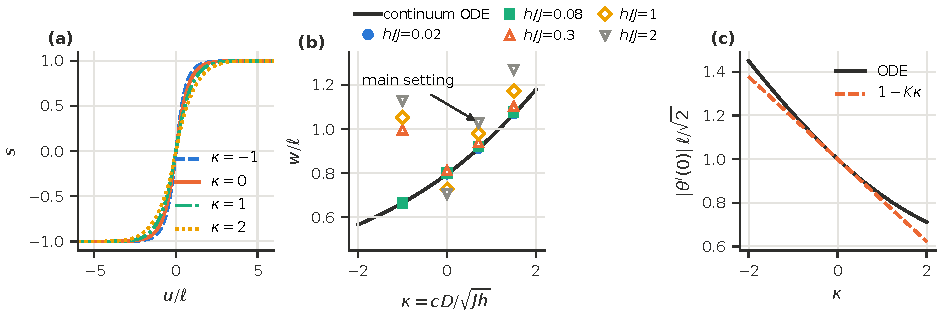
\includegraphics[width=\linewidth]{figures/Fig2_wall_theory.pdf}
\caption{\textbf{Wall widths collapse onto $w=\ell F(\kappa)$ once walls span several lattice spacings, and the chiral term widens them.} (a) Fixed-point profiles of Eq.~\eqref{eq:scaled} for four values of $\kappa=cD/\sqrt{Jh}$. (b) Width, defined as the standard deviation of $|\partial_us|$, divided by $\ell=a\sqrt{J/h}$. Line: continuum ODE; symbols: lattice update at five ratios $h/J$ (filled: $\ell\ge3.5a$; open: lattice-scale walls). The arrow marks the main setting $h/J=2$, $\kappa=0.71$. (c) Center slope from the ODE and the first-order law $1-K\kappa$, $K=2\sqrt2/15$. All results are exact computations without statistical error.}
\label{fig:wallth}
\end{figure}

\subsection{Metrication and curvature}\label{subsec:res:metric}
If walls are centered and saturated, the coarea identity leaves lattice metrication as the only source of error. We test this in two steps. \emph{Planar walls.} Straight walls with rational normals $(p,q)$ on periodic $120^2$ arrays give the metrication function $m(\varphi)$ in Fig.~\ref{fig:metric}(a). As predicted, $m=1$ to machine precision at $\varphi=0^\circ$ and $45^\circ$. In between it rises to $1.028$ for $D/J=1$ and $1.067$ for $D/J=0$, giving orientation averages $\bar m_2=1.0189$ and $1.0437$. In 3D, 40 primitive normals with $|\bm\nu|^2\le50$ on $60^3$ arrays, weighted by their Voronoi solid angles, give $\bar m_3=1.0160$. Again $m=1$ exactly for [100], [110] and [111].

\emph{Curvature.} Disks and spheres approach the planar value as $1/R\to0$ and fall below it for radii of a few lattice spacings [Figs.~\ref{fig:metric}(b) and \ref{fig:metric}(c)]. The cubic law of Eq.~\eqref{eq:mkappa} describes both within the scatter over subpixel centers. For disks with $R\ge8$, the wall offset $|\langle u\rangle|$ stays below $0.021$ pixels, so the topological Steiner term in Eq.~\eqref{eq:steiner} is negligible in 2D. In 3D the measured $\langle u^2\rangle=0.525$ voxel$^2$ predicts a positive correction of $0.53/R^2$. The observed small-radius deficit has the opposite sign, so lattice sampling of curvature, which $m_3(\kappa)$ absorbs, dominates over the continuum Steiner term.

\begin{figure}[t]
\centering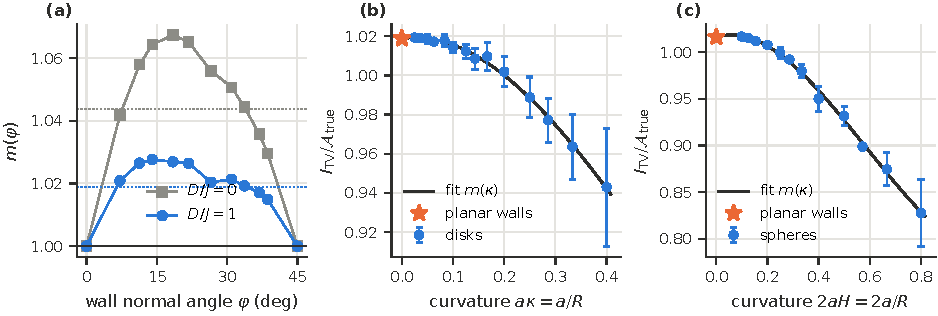
\includegraphics[width=\linewidth]{figures/Fig3_metrication.pdf}
\caption{\textbf{Lattice symmetry fixes the planar metrication, and one curvature law describes disks and spheres.} (a) $I_{\rm TV}$ per unit length of straight walls versus normal angle for $D/J=0$ and $1$; values are exact. Unity on the mirror directions $0^\circ$ and $45^\circ$ follows from telescoping; dotted lines mark the orientation averages $\bar m_2$. (b) Ratio of $I_{\rm TV}$ to the exact perimeter for disks versus curvature $a/R$, with the planar value (star) and the fitted law of Eq.~\eqref{eq:mkappa} (line). Points: means over six random subpixel centers; bars: standard deviation. (c) Same for spheres versus $2a/R$ (three centers per radius).}
\label{fig:metric}
\end{figure}

\subsection{Scale-selective filtering and noise}\label{subsec:res:noise}
The sign rule makes a sharp prediction: whether a feature survives depends only on its least-supported site and on $h/J$. Figure~\ref{fig:filter}(a) tests this on seven small features in a uniform background, for $h/J=1$, $2$, $3$ and $4.5$. For each feature, the prediction uses its least-supported site. Of the 28 feature--field combinations, 24 are strictly decided by the rule, and 23 of these behave as predicted. The exception is the $2\times2$ block at $h/J=1$: it is erased although predicted stable, because at $\ell=a$ its corners are no longer Ising-like. Marginal cases (equality in Eq.~\eqref{eq:stability}) go either way; a nine-pixel line loses only its two end pixels at $h/J=2$. Repeating the test at $D/J=0$, $1$ and $2$ gave identical outcomes except for that marginal line, confirming that filtering is controlled by $h/J$, not by $D$. Holes behave exactly like objects, as (S3) requires.

Under salt-and-pepper corruption of 12 stadium masks [Fig.~\ref{fig:filter}(b)], the planar-constant readout stays at $0.45\%$ and $0.43\%$ for flip rates of $0.2\%$ and $1\%$, with mask Dice $\ge0.999$. Raw Crofton and the $N=0$ initialization fail completely ($88\%$ and $148\%$ already at $0.2\%$), because every flipped pixel adds boundary. A $3\times3$ median filter followed by Crofton gives $1.20\%$ and $1.15\%$. With the curvature-corrected readout the errors are $0.40\%$ and $0.58\%$. At a $5\%$ flip rate, adjacent defect pairs and defects touching the boundary become common. Many of them are stable or marginal under Eq.~\eqref{eq:stability}, and the error rises to $10.0\%$, worse than the median baseline ($3.5\%$). The filtering scale is set by $h/J$ and the coordination number, so the field is not a general-purpose denoiser.

\begin{figure}[t]
\centering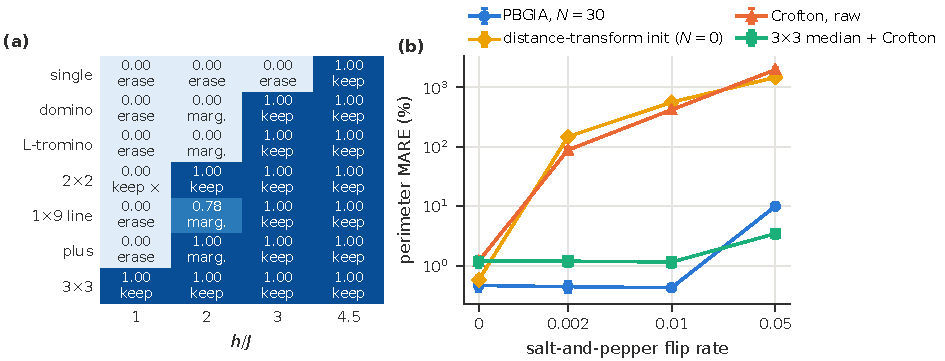
\includegraphics[width=\linewidth]{figures/Fig4_filter.pdf}
\caption{\textbf{The local sign rule predicts which features survive, which keeps perimeters accurate under sparse noise.} (a) Fraction of feature pixels whose sign survives 30 updates (color and upper number), with the prediction of Eq.~\eqref{eq:stability} for the least-supported site (lower label; ``marg.'' = equality, $\times$ = disagreement). Holes give identical results. (b) Perimeter MARE of 12 stadium shapes ($R=11$--23, three rotations; three noise realizations each) versus salt-and-pepper flip rate. PBGIA uses $I_{\rm TV}/\bar m_2$ to isolate the effect of filtering. Bars: standard error over shapes.}
\label{fig:filter}
\end{figure}

\subsection{A benchmark with exact geometry}\label{subsec:res:bench}
The tests so far isolate one mechanism at a time. A benchmark should instead combine them, with ground truth exact and comparators treated at their best. We generated shapes whose perimeters and areas are known in closed form or by converged quadrature, in seven families per dimension. In 2D these are disks, ellipses (aspect ratio 1.5--3), stadiums, thin rings (width 4--9 pixels), non-convex five-to-six-lobed ``flowers'', pairs of disks separated by 6--12 pixels, and near-touching pairs (gaps of 1--3 pixels). In 3D they are spheres, triaxial ellipsoids, capsules, solid tori (tube radius 3--6 voxels), non-convex ``bumpy'' spheres, separated pairs and near-touching pairs. Sizes are log-uniform (radius 4--26 pixels in 2D and 4--15 voxels in 3D), and every shape has a random rotation and subpixel shift ($128^2$ and $64^3$ grids). The test set contains 30 shapes per family in 2D and 12 in 3D, 294 in total, each evaluated clean and with $0.2\%$ and $1\%$ salt-and-pepper noise. A separate training set (8 and 3 shapes per family) serves only the conventional estimators. It fixes their multiplicative calibration and selects the Gaussian pre-smoothing width ($\sigma=0.75$ in 2D, $0.5$ in 3D) that minimizes their training error. PBGIA is never calibrated on these shapes. The training set is used only to choose between two theory-motivated settings by their mean error over the three noise levels: the field strength $h/J\in\{1.5,2\}$, which trades filtering of attached defects against erosion of fine lobes (Sec.~\ref{subsec:stability}), and the orientation-averaged or direction-resolved metrication. The selected readouts are $h/J=1.5$ with Eq.~\eqref{eq:mphikappa} in 2D and $h/J=2$ with Eq.~\eqref{eq:mkappa} in 3D.

Table~\ref{tab:extent} and Fig.~\ref{fig:bench} summarize the results, averaged over the six non-contact families. In 2D, PBGIA has the lowest clean error, $0.54\%$, against $0.70\%$ for calibrated Gaussian smoothing with marching squares, $0.81\%$ for calibrated Crofton and $1.17\%$ for median filtering with Crofton. The paired, family-stratified differences are significant against each comparator: $-0.15$ percentage points against Gaussian smoothing (95\% interval $[-0.22,-0.09]$) and $-0.26$ against Crofton ($[-0.38,-0.13]$). In 3D, PBGIA and calibrated marching cubes are equally accurate on clean data ($0.35\%$ each; difference $0.00$, $[-0.09,+0.09]$), and PBGIA is more accurate than Gaussian smoothing with marching cubes ($-0.21$, $[-0.31,-0.12]$). The advantage persists when the disks and spheres, the shapes from which the curvature laws were fitted, are excluded: $0.59\%$ against $0.72\%$ and $0.78\%$ in 2D, and $0.35\%$ against $0.34\%$ in 3D. Under noise, the conventional estimators fail without preprocessing ($96\%$--$541\%$). Gaussian pre-smoothing is adequate in 2D but fails in 3D at $1\%$ ($10.1\%$), and median filtering costs accuracy everywhere ($1.2\%$--$1.8\%$). PBGIA remains at $0.58\%$ and $0.81\%$ in 2D and $0.36\%$ and $0.49\%$ in 3D, the lowest values under every noise level. At the $1\%$ flip rate in 2D, it improves on Gaussian smoothing by $-0.25$ points ($[-0.40,-0.11]$). Relative to the $h/J=2$ readout, the selected 2D setting leaves clean accuracy unchanged ($-0.00$, $[-0.04,+0.03]$) and reduces the error at $1\%$ noise by $0.14$ points ($[-0.20,-0.09]$), because the weaker field removes defects attached to the boundary (Eq.~\eqref{eq:stability} with $z_{\rm in}=1$).

The theory also predicts where the readout must fail, and the benchmark finds the failures there. The largest family error in 2D is for flowers ($1.6\%$). It comes entirely from shapes whose smallest radius of curvature is below about $1.7$ pixels, beyond the range of the curvature law, where the field also erodes the tips of the lobes. The error is below $1.7\%$ for every flower with a larger radius. For near-contact pairs we varied the gap continuously [Fig.~\ref{fig:bench}(e)]. The readout is accurate to within $0.2\%$ for gaps of two pixels or more. Below that, the level sets of the two disks merge as described in Sec.~\ref{subsec:readout}, and the perimeter is underestimated by $0.6\%$ at a gap of $1.75$ pixels and by $4\%$ at one pixel. Crofton degrades only once the raster itself joins the disks. Averaged over gaps of 1--3 pixels, the near-touching family still gives $0.53\%$ (2D) and $0.44\%$ (3D).

\emph{What limits the remaining error.} Once the curvature law has removed the systematic part, the remaining error is set by the raster itself, and two results make this precise. The first is an absolute bound. For a disk of unknown center $\bm c$ and radius $R$, pixel membership is linear in $(c_x,c_y,R^2-|\bm c|^2)$, so all disks consistent with a given mask form a convex polytope. Its width in $R$ is the gap between the lattice points nearest to the circle on either side. These points have density $2\pi R$ per unit radius, so the gap is about $1/2\pi R$, and
\begin{equation}
\frac{\delta P}{P}\simeq\frac{1}{2\pi R^{2}}
\label{eq:infobound}
\end{equation}
for any estimator, even one told that the object is a disk. Sampling the polytope gives an exponent of $-2.02$ and a prefactor of $0.159$ [Appendix Fig.~\ref{fig:floor}(a)]. The second result describes a local estimator. A subpixel displacement $\delta n$ of the boundary changes the perimeter by $\delta P=\oint\kappa\,\delta n\,ds$, the first variation of length. If the displacement left undetermined by the raster is uncorrelated along the boundary, the spread over poses is
\begin{equation}
\mathrm{var}_{\rm pose}(P)=c\oint\kappa^{2}\,ds,
\label{eq:quantlaw}
\end{equation}
with $c=2/9\pi=0.071$ when every grid crossing contributes an independent uniform displacement. We rendered each 2D test geometry in 25 random poses. The PBGIA spread follows Eq.~\eqref{eq:quantlaw} (correlation $0.77$) with $c=0.050$ [Appendix Fig.~\ref{fig:floor}(b)]: the field averages neighboring crossings and does better than independent ones. Gaussian smoothing gives $c=0.057$, while the Crofton spread grows with the perimeter instead, as staircase noise. For disks, the PBGIA spread is within a factor $1.3$--$1.5$ of the bound \eqref{eq:infobound} for $R=4$--$6$ and within a factor $3.3$ at $R=26$, where both are below $0.1\%$. Over the five families other than flowers, the pose spread alone accounts for $0.28$ of the pose-averaged $0.33\%$. The residual error is thus rasterization rather than a shortcoming of the readout. Reducing it further requires either knowledge of the shape beyond local regularity or more information per pixel, such as the partial-volume input of Appendix~\ref{app:gray}.

\begin{figure}[t]
\centering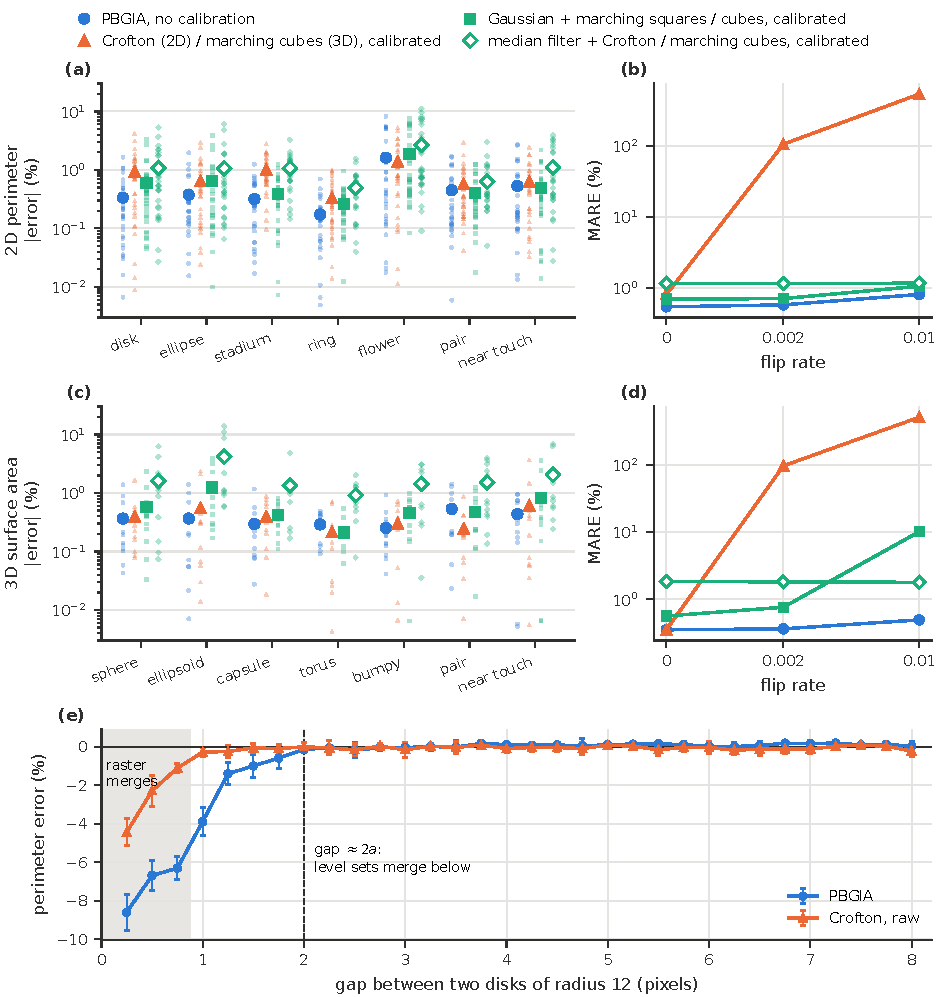
\includegraphics[width=\linewidth]{figures/Fig5_benchmark.pdf}
\caption{\textbf{Without any calibration, PBGIA is the most accurate estimator in 2D, ties calibrated marching cubes in 3D, and is the only one that stays accurate under noise without preprocessing.} (a) Clean 2D perimeter errors of the 30 test shapes per family (small symbols) and their mean (large symbols). (b) MARE over the six non-contact families versus salt-and-pepper flip rate (clean plotted at $5\times10^{-4}$). (c,d) Same for 3D surface areas (12 shapes per family). Conventional estimators are calibrated, and their Gaussian width selected, on a separate training set. (e) Perimeter error of two disks of radius 12 versus their gap, for the selected 2D readout (six random poses per gap; bars, standard deviation). Gray, gaps at which the raster joins the disks; dashed line, gap of two lattice spacings, below which the deepest level sets of the field merge.}
\label{fig:bench}
\end{figure}

\begin{table}[t]
\centering\caption{\textbf{Benchmark MARE (\%) over the six non-contact families.} 2D: 180 test shapes; 3D: 72 test shapes; each at three flip rates. Conventional estimators are calibrated on a separate training set; PBGIA is not. In 2D, Crofton and marching squares on the binary mask coincide after calibration. $^{a}$2D: $h/J=1.5$ with Eq.~\eqref{eq:mphikappa}; 3D: $h/J=2$ with Eq.~\eqref{eq:mkappa}.}\label{tab:extent}
\small\begin{tabular}{@{}lrrrrrr@{}}\toprule
 & \multicolumn{3}{c}{2D perimeter} & \multicolumn{3}{c}{3D surface area}\\\cmidrule(lr){2-4}\cmidrule(lr){5-7}
Method / flip rate & 0 & 0.002 & 0.01 & 0 & 0.002 & 0.01\\\midrule
PBGIA, no calibration$^{a}$ & 0.54 & 0.58 & 0.81 & 0.35 & 0.36 & 0.49\\
Crofton / marching cubes, calibrated & 0.81 & 106 & 539 & 0.35 & 96 & 508\\
Gaussian + marching squares / cubes, calibrated & 0.70 & 0.71 & 1.06 & 0.56 & 0.76 & 10.1\\
Median filter + Crofton / marching cubes, calibrated & 1.17 & 1.16 & 1.17 & 1.83 & 1.81 & 1.78\\\bottomrule
\end{tabular}
\end{table}

\emph{Larger shapes.} For the 27 stadium poses of Fig.~\ref{fig:stadium} ($R=9$--25, $L=2R$), the readout gives MARE $0.39\%$ (maximum $1.10\%$), against $1.13\%$ for raw Crofton. For five smooth $68^3$ volumes (sphere, capsule, solid torus, sphere pair, four fibers of radius $3.8$), it gives errors of $-0.12$, $-0.22$, $-0.14$, $+0.59$ and $-0.22\%$ (MARE $0.26\%$). Marching cubes calibrated on the sphere of the same set is slightly better here, with a MARE of $0.15\%$ on the other four. For large, clean, isolated 3D objects, a calibrated mesh estimator therefore remains the simplest choice.

\subsection{Normals, axes and projective directors}\label{subsec:res:orient}
The transverse spin should point along the inward normal, and its tensors should therefore encode orientation. On narrow boundary bands, the signed mean cosine between $\vv$ and the analytic inward normal was $0.9938$ in 2D and $0.9967$ in 3D. Axis errors from the Gram tensor were below $0.52^\circ$ for elongated 2D and 3D test shapes (Table~\ref{tab:orient}). For twelve rotations of an $R=17$ stadium, the wall-weighted spatial covariance recovered the axis with a mean error of $0.21^\circ$ [Fig.~\ref{fig:stadium}(a)]. In a synthetic four-fiber volume, the minimum-eigenvalue axis of $\int(1-s^2)\vv\vv^{\mathsf T}$ was $3.76^\circ$ from the prescribed direction. Binary PCA is equally accurate for the global axes of connected shapes. The value of the field lies in providing normals and tensors locally, which PCA does not.

\begin{figure}[t]
\centering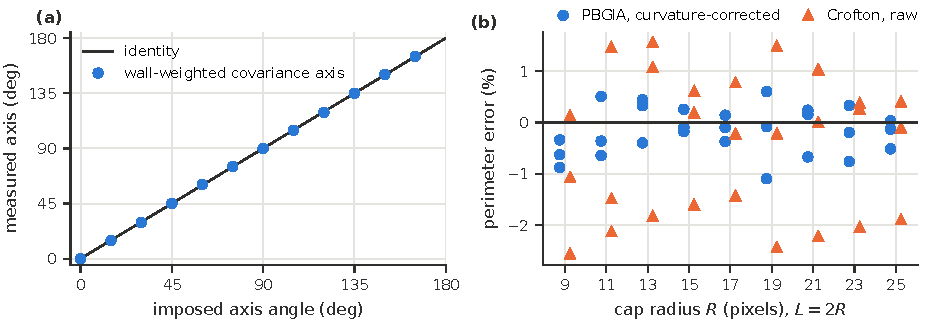
\includegraphics[width=\linewidth]{figures/Fig6_stadium.pdf}
\caption{\textbf{Axes and perimeters of rotated stadiums are recovered without calibration.} (a) Long axis from the wall-weighted spatial covariance versus imposed angle for twelve rotations of an $R=17$, $L=34$ stadium (mean error $0.21^\circ$). (b) Relative perimeter error of the curvature-corrected readout and raw Crofton for nine cap radii and three rotations each ($0^\circ$, $27^\circ$, $54^\circ$); exact perimeter $P=2\pi R+2L$. Points are offset horizontally for visibility.}
\label{fig:stadium}
\end{figure}

\begin{table}[t]
\centering\caption{\textbf{Orientation and topology readouts.} Direction errors refer to the stated geometric target.}\label{tab:orient}
\small\begin{tabularx}{\linewidth}{@{}p{.55\linewidth}X@{}}\toprule
Readout and target & Result\\\midrule
Inward-normal cosine of $\vv$ (2D/3D) & $0.9938/0.9967$\\
Gram-tensor axis error, ellipse/stadium (2D) & $0.205^\circ/0.512^\circ$\\
Gram-tensor axis error, ellipsoid/capsule (3D) & $0.332^\circ/0.385^\circ$\\
Covariance axis, separated pair (2D/3D) & $0.080^\circ/0.162^\circ$\\
Stadium covariance axis, 12 rotations & $0.214^\circ$\\
Four-fiber volume, minimum-eigenvalue axis & $3.76^\circ$\\
$Q_2$: disk / two disks / annulus / disk+annulus & $1/2/0/1$\\
$Q_3$: sphere / capsule / torus / pair / four fibers & $1/1/0/2/4$\\
$Q_3$, porous volume (generated $\chi_{26}=-5$) & $-5$\\\bottomrule
\end{tabularx}
\end{table}

\subsection{Director defects and the choice of scale}\label{subsec:res:defects}
We now turn from boundaries to textures, where the projective director and its defects are the relevant objects. \emph{Grayscale orientation.} The threshold-pooled director reproduces the orientation of synthetic and CC0 textures (Appendix Fig.~\ref{fig:gallery}). On synthetic curved strata with an analytic tangent field, its mean axial error decreases from $2.3^\circ$ at $\sigma=2$ to $0.9^\circ$ at $\sigma=16$. A direct grayscale structure tensor reaches $0.2^\circ$ at $\sigma=4$. Under imposed rotations, the structure tensor is also more consistent, both globally (Table~\ref{tab:multithresh}) and locally ($<1^\circ$ against $1$--$7^\circ$ for PBGIA over $\sigma=2$--$16$). Most of this gap is due to the threshold stack rather than to the field. When the generator is driven directly by the normalized intensity (Appendix~\ref{app:gray}), the rotation error falls on all nine textures and is within $0.1^\circ$ of the structure tensor, or better, on five (Table~\ref{tab:multithresh}). On the strata it becomes $0.20^\circ$ at $\sigma=8$, against $0.32^\circ$ for the structure tensor. The local rotational error falls from $1.0$--$6.9^\circ$ to $0.1$--$1.9^\circ$ (structure tensor $0.05$--$1.0^\circ$; Appendix Fig.~\ref{fig:contdir}). Because the structure tensor remains clearly better on the other four textures, we do not present the director as a better orientation estimator. For the defect analyses below we keep the threshold stack, which isolates the defects of a noisy texture at smaller windows (Appendix~\ref{app:gray}). What it adds is a projective field, derived from the same spin texture, whose topology and scale dependence follow Secs.~\ref{subsec:charge} and \ref{subsec:scale}.

\emph{Known defects.} To test Eqs.~\eqref{eq:charge}--\eqref{eq:annihilation}, we built a $320^2$ texture by line-integral convolution of filtered noise along a director field with four prescribed disclinations: a close pair ($\pm\tfrac12$, $d=40$ pixels) and a far pair ($d=110$) [Figs.~\ref{fig:defects}(a)--\ref{fig:defects}(c)]. At small $\sigma$ the pixel-level field is dominated by noise, and defects of both signs proliferate in equal numbers. For $6\le\sigma\le14$, PBGIA finds exactly the four prescribed defects with correct signs, within a few pixels of their positions; the structure tensor does so for $4\le\sigma\le16$. The close pair annihilates between $\sigma=16$ and $18$, as Eq.~\eqref{eq:annihilation} predicts ($0.4413\times40=17.7$). The far pair disappears between $\sigma=40$ and $50$ (predicted $48.5$). The net charge in the region stays zero throughout, as conservation (i) requires. The anisotropy around an isolated core follows the exact law \eqref{eq:core} for all windows [Fig.~\ref{fig:defects}(h); maximum deviation $0.03$].

\emph{Real texture and the role of $\sigma$.} The CC0 grass image (the texture on which the global axis readout failed) shows why the window must be chosen rather than fixed [Figs.~\ref{fig:defects}(d)--\ref{fig:defects}(g)]. At $\sigma=2$--$4$ the director follows individual blades, and hundreds of $\pm\tfrac12$ defects mark where blades cross or end. At $\sigma=8$, the window used in the gallery, most of this local structure is averaged away, and at $\sigma=16$ only a few patches of coherent orientation remain. The defect count measures this quantitatively [Fig.~\ref{fig:defects}(i)]. For grass it follows the parameter-free random-field law \eqref{eq:randomdensity} within a factor $0.74$--$1.0$ over $\sigma=2$--$16$: beyond the blade width, its orientation is statistically random at every scale. Brick and wood fall below the law and become defect-free for $\sigma\ge12$, the signature of long-range order. The weave exceeds the law up to its period, because its crossing points form a lattice of defects, and drops below it beyond. The retinal image lies in between. A single orientation map at one fixed $\sigma$ hides these differences; the scale dependence of the defect density reveals them.

\begin{figure}[t]
\centering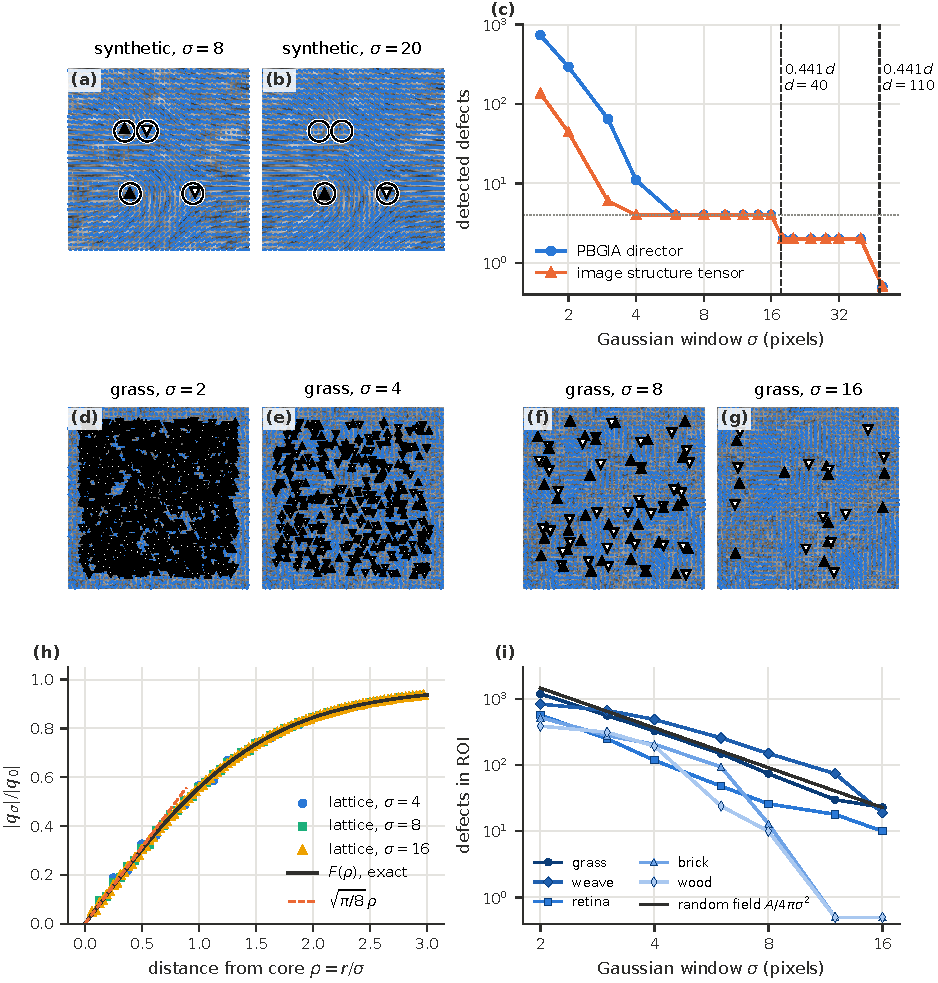
\includegraphics[width=\linewidth]{figures/Fig7_director_defects.pdf}
\caption{\textbf{Half-integer defects of the projective director are conserved across scales, annihilate at the predicted window, and measure orientational disorder.} (a,b) Synthetic texture with four prescribed disclinations (open circles) and the PBGIA director at $\sigma=8$ and $20$; detected $+\tfrac12$ (filled up-triangles) and $-\tfrac12$ (open down-triangles) defects. (c) Number of detected defects versus $\sigma$; dashed lines, predicted annihilation scales $0.4413\,d$ for the two pairs; zero is plotted at $0.5$. (d--g) CC0 grass texture with directors and defects at four windows. (h) Anisotropy around an isolated defect versus $r/\sigma$ for three windows, with the exact law of Eq.~\eqref{eq:core}. (i) Defects in a $271^2$-pixel region versus $\sigma$ for five textures, with the random-field law $A/4\pi\sigma^2$ (line, no fit); zero is plotted at $0.5$.}
\label{fig:defects}
\end{figure}

\subsection{Topology of the generated field}\label{subsec:topo}
Equation~\eqref{eq:hopf} predicts that the degree counts the topology of the generated domain, which coincides with the input only when nothing is filtered. For four 2D masks (disk, two disks, annulus, disk plus annulus), the spherical-triangle charge of the actual 30-step fields was $Q_2=1,2,0,1$ to within $2\times10^{-8}$, equal to the Euler characteristics [Figs.~\ref{fig:topology}(a)--\ref{fig:topology}(d)]. In 3D, regular-value counts gave $Q_3=1,1,0,2,4$ for sphere, capsule, solid torus, sphere pair and four fibers, identically for three generic targets. For these smooth shapes the generator changed no voxel, so input and generated topology coincide.

The porous volume (a Gaussian random field inside a ball, $68^3$) is the informative case [Fig.~\ref{fig:topology}(h)]. It gives $Q_3=-5$. Its input mask is topologically ambiguous: $\chi=-4$ with six components under 6-connectivity, and $\chi=-6$ with two components under 26-connectivity. The input contains four isolated voxels and a 41-voxel fragment. By Eq.~\eqref{eq:stability} with $h=2J<6J$, isolated voxels must disappear, and the generator changes 231 voxels (188 removed, 43 added). The generated domain $\{s>0\}$ is a single component with $\chi_{26}=-5$, exactly the measured degree. The degree is thus a correct invariant of the filtered field. The apparent mismatch reflects scale-selective filtering together with the convention dependence of digital topology, not an error of the degree evaluation. Because the regular-value count passes many near-degenerate tetrahedra in this volume, values for such complex volumes should be accompanied by an interpolation-regularity check.

\begin{figure}[t]
\centering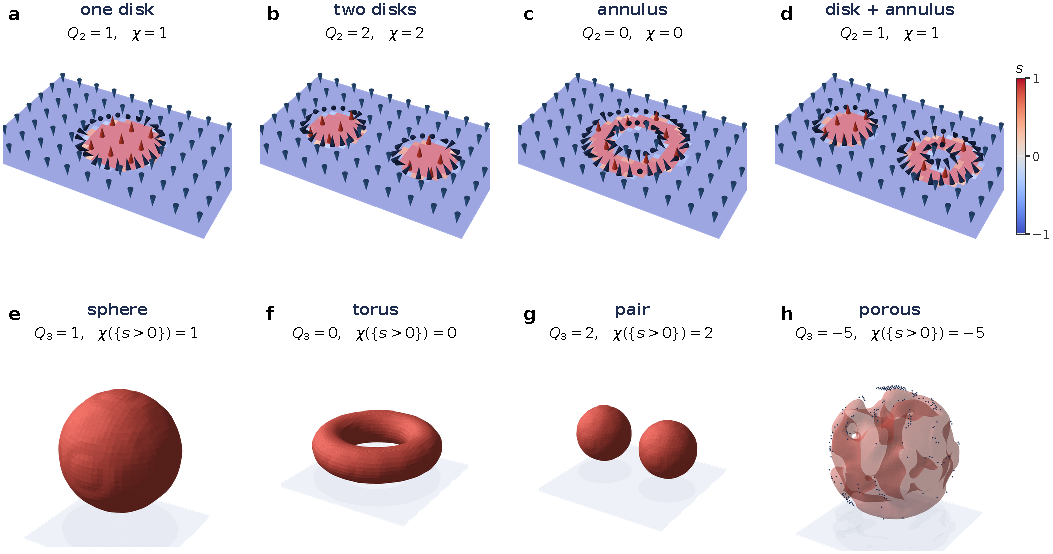
\includegraphics[width=\linewidth]{figures/Fig8_topology.pdf}
\caption{\textbf{The integer degree of the generated field equals the Euler characteristic of the generated domain, including when filtering changes the input.} (a--d) Generated $s$ for four 2D masks with the spherical-triangle charge $Q_2$ and the raster Euler characteristic. (e--h) Central slices of generated $s$ for 3D volumes with the regular-value degree $Q_3$ and $\chi$ of $\{s>0\}$ (26-connectivity). In (h), open black squares mark input voxels removed by the generator in this slice. All values are exact integers; $N=30$.}
\label{fig:topology}
\end{figure}

\FloatBarrier
\subsection{Magnetic domain images}\label{subsec:res:magnetic}
The representation was motivated by magnetization, so magnetic images are a natural test. We analyzed three published experimental data sets (Fig.~\ref{fig:magnetic}).

\emph{Skyrmion lattice.} The first is a Lorentz transmission electron micrograph of a N\'eel skyrmion lattice ($1024^2$ pixels)~\cite{McCray2024}. For a tilted sample, the Lorentz contrast of N\'eel skyrmions is approximately a directional derivative of $m_z$ along the tilt axis. We estimated that axis from the anisotropy of the power spectrum (ratio $3.1$) and integrated along it in Fourier space with Tikhonov regularization. Each skyrmion then appears as a compact bright disk [Fig.~\ref{fig:magnetic}(b)]. The first Bragg ring gives a lattice spacing of $29.8$ pixels. The generated field was cut at a quantile of the normalized map, and the number of $s>0$ domains in the central $928^2$ region stays between $1067$ and $1082$ for cut quantiles $0.70$--$0.85$ [inset of Fig.~\ref{fig:magnetic}(c)]. At $0.75$ it is $1074$, which is $4\%$ below the $1120$ expected for an ideal triangular lattice of this spacing; a Laplacian-of-Gaussian blob detector applied to the same map finds $1144$. The degree tests the topological readout directly. Summing the charge density over the Voronoi cell of each domain gives $Q=1.0000\pm0.0015$ per domain; the largest deviation from unity is $0.026$, and the total over the region is $1075.2$ [Fig.~\ref{fig:magnetic}(c)]. By Hopf's theorem (Sec.~\ref{subsec:degree}), each skyrmion is a disk of the generated domain and contributes exactly one unit of degree. The transverse spin therefore introduces no spurious winding, even on a noisy experimental map, and the degree counts skyrmions.

\emph{Labyrinth domains.} The second data set is a Kerr image of a labyrinth domain pattern ($256^2$ pixels, stripe period $10.7$ pixels from the power spectrum), together with the authors' binarization~\cite{Zhao2026}. A labyrinth provides an independent morphological ground truth for the director charges of Sec.~\ref{subsec:charge}. A stripe end is a $+\tfrac12$ disclination of the stripe director, and a three-fold branch point is a $-\tfrac12$ disclination, in either phase. We counted both on pruned skeletons of the authors' binary image, which gives 489 ends and 615 branch points in the analyzed region. The PBGIA director was computed from the raw image with the continuous source, and its plaquette charges were compared with these features [Fig.~\ref{fig:magnetic}(e)]. Because the defects are dense, a loose matching radius is met by chance, so we report two controls: the same number of defects placed at random, and the detected defects with their signs exchanged [Fig.~\ref{fig:magnetic}(f)]. At $\sigma=1.5$ and a matching radius of two pixels, $42\%$ of the 1148 detected defects coincide with a feature of the same sign. Random placement gives $12\%$ and sign exchange $7\%$, so the matches are three to six times above chance and strongly sign-specific. The recall is $43\%$. The structure tensor at the window that yields the same number of defects gives $39\%$ and $43\%$. The skeleton reference is itself imperfect, because the binarization keeps pixel-scale roughness that creates spurious ends and branch points; the agreement is therefore a lower bound. The charges of the director field thus correspond, sign by sign, to the stripe ends and branch points that define the labyrinth's topology.

\emph{Bubble growth under field pulses.} The third data set consists of two Kerr-microscopy sequences of a single bubble domain growing under repeated field pulses (nine frames each, $1344\times1020$ pixels, $0.32\,\mu$m per pixel)~\cite{KerrPy}. We used difference images against the saturated state. Their per-pixel contrast-to-noise ratio is only $0.72$ and $0.78$, so no raw-pixel method can work [Fig.~\ref{fig:magnetic}(d)]. The sign rule turns this into a choice of scale. A mid-level cut of an image smoothed with a Gaussian of width $\sigma$ flips a fraction $\Phi(-\mathrm{SNR}_\sigma/2)$ of plateau pixels, where $\mathrm{SNR}_\sigma=2\sqrt\pi\,\sigma\,\mathrm{SNR}_1$ for white noise. Eq.~\eqref{eq:stability} removes such flips only while they are isolated. We therefore took the smallest $\sigma$ for which this fraction is at most $0.3\%$, which gives $\sigma=2.5$ and $2.0$ pixels for the two sequences, with no tuning. With this $\sigma$, the PBGIA readout and Gaussian smoothing with marching squares agree to within $0.4\%$ in area and $1.8\%$ in perimeter (mean $0.8\%$) over all frames, and both follow the growth smoothly. A residual from a cubic fit in pulse number is $1.2$--$1.3\%$ for PBGIA and $1.3$--$1.5\%$ for Gaussian smoothing [Fig.~\ref{fig:magnetic}(f)]. A median-filter and Otsu pipeline of the kind used for such data returns perimeters $1.3$ to $3.0$ times larger, fluctuating by $11$--$17\%$ between pulses, because it keeps the roughness of the noisy boundary. On these images PBGIA is not more accurate than Gaussian smoothing at the same width; what the theory contributes is the width itself.

\begin{figure}[t]
\centering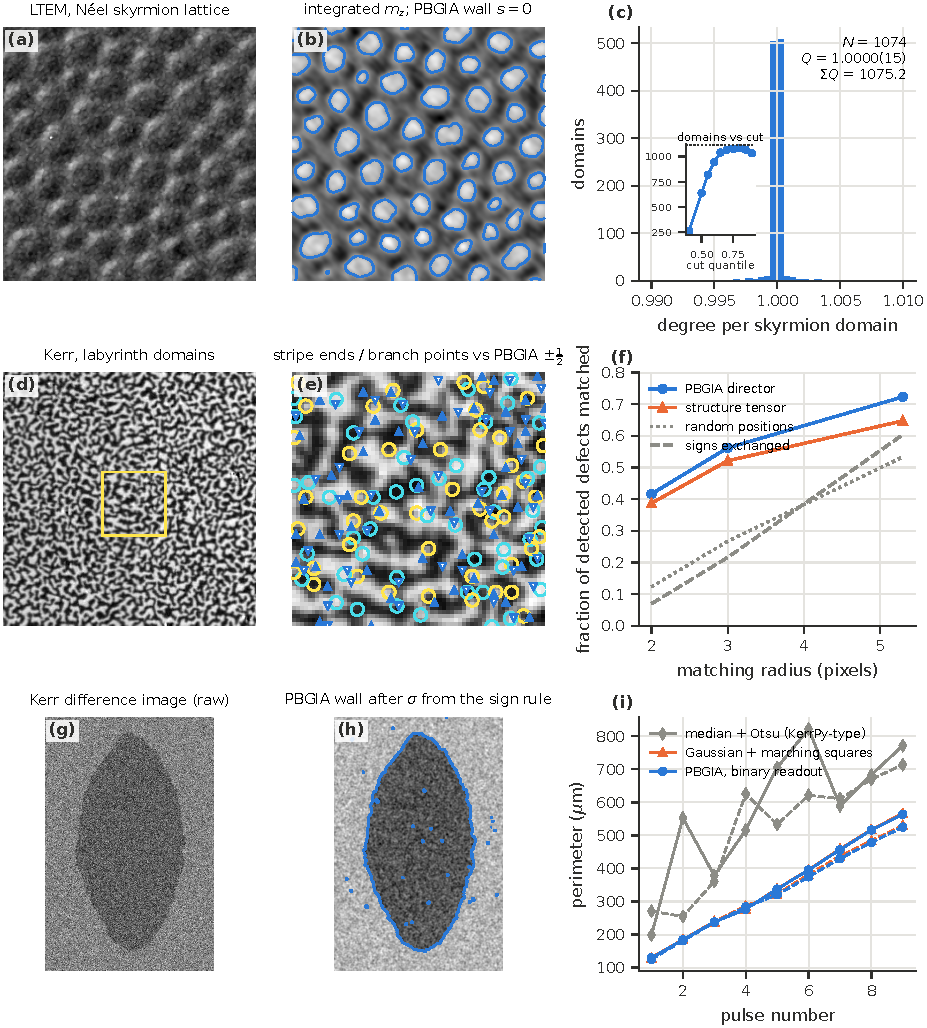
\includegraphics[width=\linewidth]{figures/Fig9_magnetic.pdf}
\caption{\textbf{On experimental magnetic images, the degree counts skyrmions, the director charges mark stripe ends and branch points, and the sign rule fixes the smoothing scale.} (a) Lorentz micrograph of a N\'eel skyrmion lattice (detail, $220^2$ pixels; data of Ref.~\cite{McCray2024}). (b) The same region after integration along the tilt axis, with the wall $s=0$ of the generated field (blue). (c) Degree summed over the Voronoi cell of each of the $1074$ domains in the central region. Inset: number of domains versus cut quantile; dotted line, ideal triangular lattice. (d) Kerr image of labyrinth domains (data of Ref.~\cite{Zhao2026}); the box marks the region enlarged in (e). (e) Stripe ends (yellow circles, $+\tfrac12$) and branch points (cyan circles, $-\tfrac12$) from skeletons of the authors' binarization, with the PBGIA director defects at $\sigma=1.5$ (filled triangles, $+\tfrac12$; open triangles, $-\tfrac12$). (f) Fraction of detected defects that lie within the matching radius of a feature of the same sign, for PBGIA and the structure tensor at windows giving about $1150$--$1200$ defects, with two chance controls. (g) Kerr difference image of a growing bubble domain (data of Ref.~\cite{KerrPy}), unsmoothed. (h) The same image smoothed with the width chosen by the sign rule ($\sigma=2$), with the PBGIA wall; the small isolated contours are surviving noise clusters outside the domain. (i) Perimeter versus pulse number for the two sequences (solid and dashed).}
\label{fig:magnetic}
\end{figure}

\section{Discussion}\label{sec:discussion}
The starting idea was that an image, read as a magnetic field, induces a magnetization whose structure encodes the image's geometry. The results show that this idea is more than a metaphor. Once the actual alignment rule is treated as the physical system, each geometric readout rests on a specific mechanism with a checkable assumption.

\emph{Where the assumptions hold, and why.} The wall theory assumes only that fixed points align each spin with its local field. This is exact for the rule, even though no energy exists. The continuum equation \eqref{eq:fixedODE} then follows, and the observed collapse of wall widths for $\ell\gtrsim3.5a$ confirms that the chiral coupling enters only through $\kappa$. The filtering law assumes Ising-like neighbors. This is accurate precisely in the lattice regime used in practice, where walls are one spacing wide, and there it predicts which features survive without any fitted constant. The boundary readout assumes that walls saturate and are centered. Both properties follow from the wall theory, so the residual error is lattice metrication. Symmetry reduces this to one planar constant and a smooth function of curvature, and a law determined on disks and spheres transfers to ellipses, capsules, tori and rings that it has never seen. The degree assumes that the transverse spin on the zero set follows the inward normal. Hopf's theorem then makes the degree the Euler characteristic of the generated domain, and the porous volume shows that this identification is exact even when filtering changes the input.

\emph{Where the method must fail.} The same assumptions predict the failures. Saturation breaks down between objects closer than a wall width: their deeper level sets merge, and the facing boundaries are undercounted. The sign rule cannot distinguish a one-site defect from a one-site feature, so it removes both. At high defect densities, clusters become stable under the rule and survive. In each case the failure follows from a formula, and the benchmark finds it where the formula places it: for gaps below about two lattice spacings and for curvature radii below about two spacings. In our view, this predictive account of failure is the strongest argument for the approach.

\emph{Three scales.} The theory separates three length scales that a practitioner can set independently. The ratio $h/J$ sets the smallest feature that survives, $\kappa$ sets the wall width and thereby the metrication error, and the Gaussian window $\sigma$ sets the scale at which orientation is reported. The third is of a different nature: it acts on the projective director rather than on the generator. Because charge is conserved across windows, a scan over $\sigma$ adds or removes only neutral defect pairs. The resulting defect density, compared with the random-field value $1/4\pi\sigma^2$, gives a compact description of orientational order across scales. For the grass texture, this description shows directly what a single fixed window had hidden.

\emph{Relation to conventional estimators.} Without any calibration, the readout is more accurate than calibrated contour estimators in 2D and as accurate as calibrated marching cubes in 3D. It is the most accurate estimator under sparse noise, because the sign rule removes defects that every raster method counts as boundary. These gains have identifiable origins. Lattice symmetry and the curvature law replace an empirical calibration, the coarea average over level sets replaces a single staircase contour, and the filtering is built into the generator. For large, clean, isolated 3D objects, a calibrated mesh estimator remains an equally good and simpler choice, and a grayscale structure tensor gives better local orientation. The field's further value is that extent, normals, director topology and degree come from one representation. We regard these advantages as consequences of the theory, not as the paper's main claim.

\emph{Grayscale and color images.} The source term is where intensity enters the generator, and its form follows from a conservation argument rather than from choice. A linear map of the normalized intensity is the only map that preserves the zeroth moment of a subpixel step, and by the layer-cake identity it is the average of the binary sources over all thresholds. Driven this way, the generator reduces the perimeter error of a single cut by about $40\%$ on partial-volume images and its pose variance fourfold, and it keeps the noise robustness of the binary field. On clean grayscale images, a plain marching-squares contour remains more accurate (Appendix~\ref{app:gray}). The same source closes most of the gap between the PBGIA director and the structure tensor. It does not, however, replace the threshold stack. On a noise-carrying texture with four known disclinations, the stack isolates them at smaller windows. This advantage does not come from the sign rule: filtering every threshold level before recombining them leaves the continuous result unchanged. Part of it is weighting. By the coarea formula, a dense stack weights each pixel by the density of level crossings, $|\nabla s|$. Weighting the continuous tensor in the same way improves it on every test, including orientation accuracy and defect isolation, but part of the gap at small windows remains (Appendix~\ref{app:gray}). For color images, the right reduction depends on the readout. An extent measurement needs the projection with the largest contrast-to-noise ratio, which for a two-phase image is the first principal axis of the pixel colors. Orientation, where different channels can carry different structures, needs channel-wise fields pooled as tensors. Luminance alone discards isoluminant boundaries entirely.

\emph{Limitations and outlook.} The quantitative benchmarks are synthetic; the real images, CC0 textures and three published magnetic data sets, have no external labels. The benchmark contains 294 synthetic test shapes with exact measures; images whose geometry is known independently, such as micro-CT phantoms, remain to be analyzed. The constants of the curvature law are specific to the generator parameters and to cubic lattices. Natural extensions follow from the theory itself: director defects in three dimensions, classified by $\pi_1(\RP^2)$ and $\pi_2(\RP^2)$; generators with a tunable $\kappa$ for wider, better-sampled walls; and measured partial-volume data, for which the continuous source of Appendix~\ref{app:gray} is the natural input.

\section{Methods and reproducibility}\label{sec:methods}
\emph{Generator.} Equations~\eqref{eq:updatev}--\eqref{eq:updaten} use float32 arrays, periodic boundaries, $2d$ axial neighbor sums (never replaced by a Laplacian), a centered scalar gradient, and $N=30$ synchronous updates without adaptive stopping. Initialization uses only the binary distance transform, as stated in Sec.~\ref{sec:model}.

\emph{One-dimensional walls.} Lattice walls used open chains of length $\max(200,40\ell(1+|\kappa|))$ with fixed end spins, iterated to a maximum change below $10^{-13}$. ODE profiles were obtained by bisection on the center slope with $\theta(0)=\pi/2$ (tolerance $10^{-11}$). Width is the standard deviation of $|\partial_us|$.

\emph{Metrication constants.} 2D: twelve primitive normals $(p,q)$ from $0^\circ$ to $45^\circ$ on $120^2$ periodic arrays. The mask is $((-px+qy)\bmod 120)<60$, so the total boundary length is exactly $2\cdot120\sqrt{p^2+q^2}$. $\bar m_2$ is the trapezoidal average over angle. 3D: 40 primitive normals in the fundamental wedge on $60^3$ arrays, weighted by Monte Carlo Voronoi solid angles. All gradients in these tests are periodic centered differences.

\emph{Curved shapes and noise.} Disks used grids of side $2R+30$ with eight uniformly random subpixel centers per radius. Spheres used grids of side $2R+20$ with four random centers. Stadiums used $160^2$ grids, cap radius $R$ and straight length $L=2R$. Salt-and-pepper noise flipped each pixel independently. The median baseline is a $3\times3$ median filter followed by four-direction Crofton (\texttt{scikit-image}). 3D test shapes and marching-cubes areas follow the generator in \texttt{code/new\_quantitative\_studies.py}.

\emph{Curvature law.} Disks (radii $2.5$--$40$, six random centers each) and spheres ($2.5$--$20$, three centers each) were generated with the main setting. The coefficients of Eq.~\eqref{eq:mkappa} were obtained by least squares with the constant term fixed to $\bar m_d$. Curvature is clipped at $0.45$ (2D) and $0.85$ (3D), the largest values sampled.

\emph{Readout selection.} Planar walls for Eq.~\eqref{eq:mphikappa} use all coprime $(p,q)$ with $0\le p\le q\le12$ on $240^2$ periodic arrays. Candidate settings, evaluated on the training set only, were $h/J\in\{0.7,1,1.5,2,2.5,3\}$, $D/J\in\{0.5,1,2,3\}$, stencil weights $\alpha\in\{0,0.125,0.25\}$ (2D) and $\{0,0.05,0.1\}$ (3D), and orientation-averaged or direction-resolved metrication; a 3D law including Gaussian curvature, calibrated on spheres and cylinders, was also tested. Each candidate's constants were refitted from planar walls, disks and spheres before evaluation. The test set was evaluated once with the selected settings.

\emph{Benchmark.} Exact perimeters use the complete elliptic integral for ellipses and quadrature of $\int\sqrt{r^2+r'^2}\,\dd\theta$ for flowers, $r=R(1+\epsilon\cos k\theta)$ with $k=3$--$6$ and $\epsilon=0.08$--$0.18$. Exact areas use Legendre's formula for triaxial ellipsoids, $4\pi^2Rr$ for tori, and converged quadrature for bumpy spheres, $r=R(1+\epsilon\sin^2\theta\cos3\phi)$ with $\epsilon=0.08$--$0.15$. Masks are point-sampled at pixel or voxel centers. Crofton uses four directions (\texttt{scikit-image}); marching squares and marching cubes extract the $0.5$ level of the binary or Gaussian-smoothed mask. Each conventional estimator is multiplied by the median ratio of truth to estimate on the clean training set (non-contact families). The Gaussian width is chosen from $\{0.5,0.75,1,1.5,2\}$ (2D) or $\{0.5,0.75,1,1.5\}$ (3D). Paired differences are bootstrapped within families (4000 draws), and the family means are then averaged. The gap sweep uses two disks of radius 12 at 32 gaps and six random poses per gap.

\emph{Rasterization floor.} For each radius ($R=4$--$26$, 16 random centers), the bounding box of the consistent polytope in $(c_y,c_x,R^2-|\bm c|^2)$ was found by linear programming over the pixels within two spacings of the circle and sampled uniformly until at least $3000$ consistent points were collected. Weights $1/R$ convert this sampling to a uniform prior in $R$. Pose ensembles re-render each non-contact 2D test geometry with 24 additional random rotations and subpixel shifts; the disk sweep uses 48 poses per radius.

\emph{Magnetic images.} The Lorentz image is the demonstration file of Ref.~\cite{McCray2024} (MIT licence). Its power spectrum was evaluated for $0.5k_0<|\bm k|<2k_0$ around the radial peak $k_0$, with spacing $a=2/(\sqrt3k_0)$. The integration used the filter $-ik_u/(k_u^2+\epsilon^2)$ with $\epsilon=0.25k_0$, a high-pass at $0.35k_0$ and a final Gaussian of $1.5$ pixels. The normalized map $g$ (2\%--98\% quantiles) drove the continuous source shifted to the cut level, $f=\mathrm{clip}[2(g-c)/\max(c,1-c)]$, with $h/J=2$. Domains are counted by centroid in the region $48$ pixels from the border. The labyrinth image and its binarization are the 10$^\circ$-tilt crops of Figure~6 of Ref.~\cite{Zhao2026} (CC-BY~4.0). Skeletons of both phases were pruned of spurs shorter than half a period; ends are skeleton pixels with one neighbor, and branch points are centroids of clusters of pixels with three or more. Only features at least 16 pixels from the border were used, and each feature was matched to at most one defect of the same sign. The Kerr frames are those of Ref.~\cite{KerrPy} (GPL-3.0). Contrast and noise were estimated once per sequence, on its last frame, from the class medians of an Otsu split of a smoothed copy. Area and perimeter refer to the largest domain, with the readout restricted to a band of $\pm4$ pixels around its hole-filled boundary.

\emph{Director scale space and defects.} The pixel-level tensor field $q_0$ was computed once per image from the five threshold fields and then smoothed with Gaussian windows $\sigma=1.5$--$50$ (reflecting boundaries). Defects are plaquettes with $k_p\neq0$ in Eq.~\eqref{eq:latticecharge}, counted in the central $271^2$ region. The synthetic texture is a line-integral convolution of Gaussian-filtered noise ($\sigma_n=0.9$ pixels) over $\pm14$ steps along $\psi=\sum_jk_j\arg(\bm x-\bm x_j)$, with $k_j=\pm\tfrac12$ at the four prescribed cores. A detected defect matches a prescribed one if it has the same sign and lies within $\max(6,\sigma)$ pixels. The core law was checked on the analytic field $q_0=e^{i\theta}$ on $512^2$ grids, and the annihilation constant by bisection on lattices with $d=8$--$48$ and by quadrature of Eq.~\eqref{eq:annihilation}. Local rotational consistency compares $q_\sigma$ of an image with that of the image rotated by $10^\circ$, after rotating back and removing the phase $e^{2i\cdot10^\circ}$, weighted by $|q_\sigma|$ of both.

\emph{Degree.} Spherical-triangle solid angles $\Omega=2\operatorname{atan2}[a\cdot(b\times c),1+a\cdot b+b\cdot c+c\cdot a]$ for 2D. Regular-value preimage counts on six oriented Freudenthal tetrahedra per voxel cell, after a three-voxel outer collar is set to the south pole, for 3D.

\emph{Multithreshold textures.} Inputs are rescaled to $320^2$, smoothed with $\sigma=0.8$ pixels, and thresholded at the 15, 32.5, 50, 67.5 and 85\% intensity quantiles; tensors are pooled with $\sigma=8$ pixels. Real images are \texttt{scikit-image} CC0 samples \cite{VanderWalt2014}.

\section{Conclusion}\label{sec:conclusion}
Reading a binary image as a magnetic field turns geometric measurement into a problem of magnetization structure. The alignment rule that generates this structure has no energy function, yet its fixed points are analyzable: walls obey an exact scaling law, an exact sign rule sets what is filtered, the coarea formula and lattice symmetry fix how boundaries are measured, and the projective director and the spin degree carry two distinct kinds of topology with exact laws of their own. Every readout of the field can therefore be traced to a mechanism, and every failure to a violated assumption. We expect this combination of a physical representation with a derivable error model to be the main value of the approach, beyond the particular accuracies reported here.

\section*{Data and code availability}
All code, generated data and figure scripts are available at \url{https://github.com/cywon-commits/Physics-Based-Geometric-Image-Analysis}. The generator, readout and benchmark are in \texttt{code/revision2/}, numerical results in \texttt{data/revision2/}, and figure scripts with a shared style file in \texttt{figures\_src/}. The experimental magnetic images are third-party data: the Lorentz micrograph is distributed with the SkyrmNet demonstration code of Ref.~\cite{McCray2024} (MIT licence) the labyrinth image with the data set of Ref.~\cite{Zhao2026} (CC-BY 4.0), and the Kerr sequences with KerrPy~\cite{KerrPy} (GPL-3.0).

\section*{Acknowledgments}
\emph{Funding acknowledgement to be confirmed by the author team.}

\section*{Author contributions}
\emph{To be completed with the authors' approval.}

\section*{Declaration of interests}
\emph{To be completed and confirmed by all authors.}

\section*{Use of generative AI}
AI-assisted tools were used for computational scripting, analysis and manuscript drafting. All authors must independently review and approve the final text, data and conclusions, following the selected journal's policy.

\clearpage
\appendix
\section{Supplementary figures and tables}
\begin{figure}[h]
\centering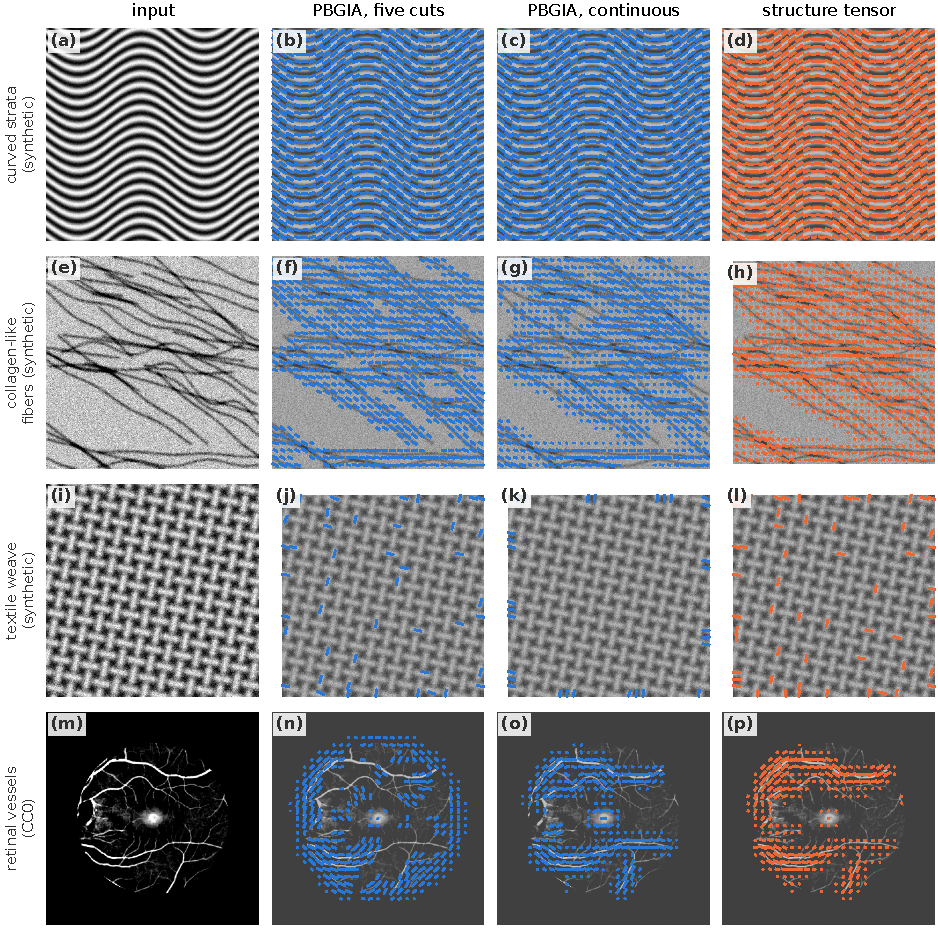
\includegraphics[width=.74\linewidth]{figures/FigA1_gallery.pdf}
\caption{\textbf{On strongly oriented textures the PBGIA director agrees with the structure tensor; on weakly oriented ones both become sparse.} Rows: synthetic curved strata (analytic tangent field available), synthetic collagen-like fibers, a synthetic weave, and a CC0 retinal image. Columns: input (contrast-stretched for display only); PBGIA director pooled over five quantile thresholds; PBGIA director from the continuous source (Appendix~\ref{app:gray}); direct grayscale structure tensor. Segment length is proportional to the normalized eigenvalue gap; window $\sigma=8$ pixels. Results for all nine textures are in Table~\ref{tab:multithresh}.}
\label{fig:gallery}
\end{figure}

\begin{figure}[h]
\centering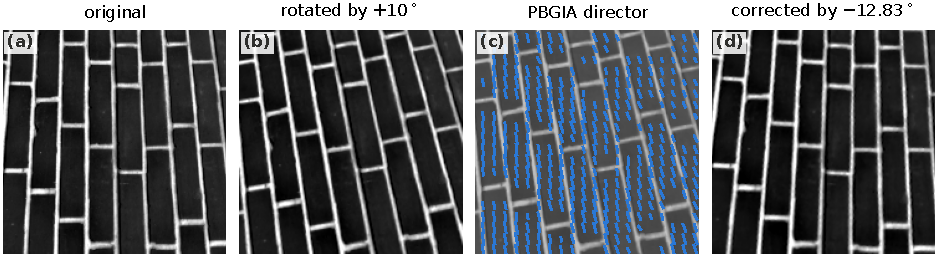
\includegraphics[width=\linewidth]{figures/FigA2_deskew.pdf}
\caption{\textbf{The pooled director tracks an imposed rotation of a real texture.} (a) CC0 brick texture; (b) the same texture rotated by $+10^\circ$; (c) PBGIA director of the rotated image; (d) rotated image corrected by the inferred $-12.83^\circ$. All panels show the same central $180\times180$-pixel window, which excludes the borders affected by rotation. The test measures rotational consistency, not absolute orientation; the residual $2.8^\circ$ lies within the rotation-tracking errors of Table~\ref{tab:multithresh}.}
\label{fig:deskew}
\end{figure}

\begin{table}[h]
\centering\caption{\textbf{The threshold stack, not the field, limits the rotational consistency of the PBGIA director.} Mean absolute error of the inferred relative axis shift over seven rotations ($-15^\circ$ to $+15^\circ$). Cuts: five quantile thresholds; continuous: normalized intensity as source (Appendix~\ref{app:gray}); ST: direct grayscale structure tensor.}\label{tab:multithresh}
\small\begin{tabular}{@{}lrrr@{}}\toprule
Texture & PBGIA, cuts & PBGIA, continuous & ST\\\midrule
Synthetic curved strata & 1.80 & 0.16 & 0.22\\
Synthetic collagen-like fibers & 0.43 & 0.36 & 0.22\\
Synthetic leaf-vein analog & 1.15 & 0.31 & 0.45\\
Synthetic wood grain & 1.42 & 0.03 & 0.23\\
Synthetic textile weave & 3.96 & 3.83 & 0.86\\
Synthetic building array & 2.91 & 0.58 & 0.51\\
CC0 brick wall & 2.46 & 1.07 & 0.74\\
CC0 retinal image & 1.22 & 0.75 & 0.72\\
CC0 grass texture & 22.76 & 3.09 & 0.49\\\bottomrule
\end{tabular}
\end{table}





\begin{figure}[h]
\centering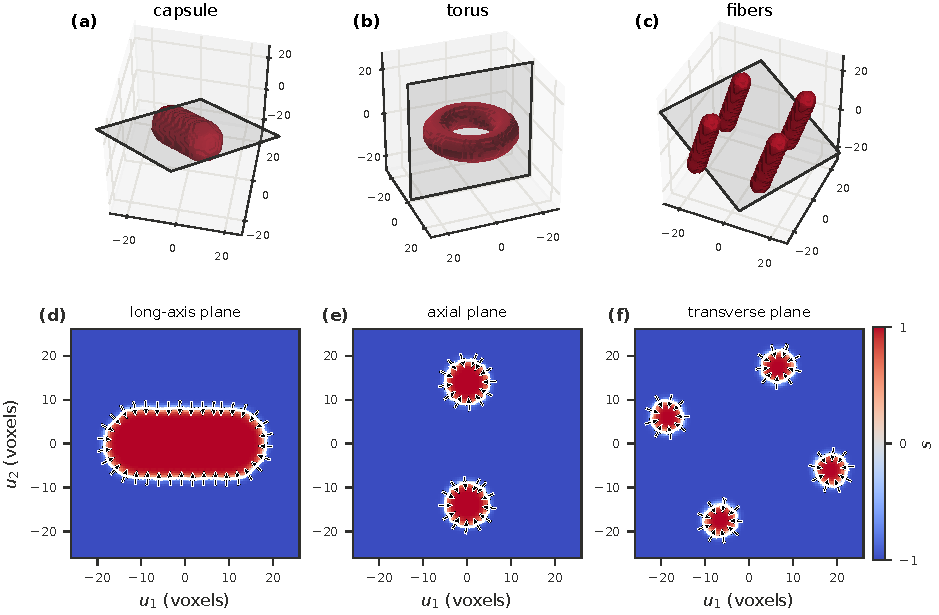
\includegraphics[width=\linewidth]{figures/FigA3_S3_field.pdf}
\caption{\textbf{In 3D the transverse part of the $\Sn^3$ spin points along the inward normal of the interface, as in 2D.} (a--c) Interface $s=0$ of the generated field for a capsule, a solid torus and four parallel fibers ($68^3$, $N=30$), with the cutting plane used below (gray). (d--f) The field on that plane: color, scalar component $s$ (shared bar); white line, $s=0$; arrows, unit projection of $\vv$ onto the plane, drawn every $2.6$ voxels along the white line. The cuts contain the capsule's long axis (d), the torus symmetry axis (e, two cross-sections of the tube), and are perpendicular to the fibers (f). In every cut the arrows point inward, so the 2D picture of Fig.~\ref{fig:concept}(c) holds on any plane through a 3D object.}
\label{fig:3Dvis}
\end{figure}

\FloatBarrier
\section{Distinct notions of topology}\label{app:topology}
The pointwise spin in $\Sn^d$, its projective class in $\RP^d$, the transverse director in $\RP^{d-1}$, the eigenline of a fiber-averaged tensor, and the Euler characteristic of a digital object are different mathematical objects. A fiber-averaged tensor can develop eigenvalue degeneracies and director defects without any singularity of the spin. Winding in $\pi_1(\RP^1)\cong\mathbb Z$ differs from the $\mathbb Z_2$ loop classification of $\RP^m$ for $m\ge2$. The compactified degree belongs to $\pi_d(\Sn^d)\cong\mathbb Z$ and is an invariant of the generated field \cite{Mermin1979}. In 3D the normal director takes values in $\RP^2$, which supports point defects classified by $\pi_2(\RP^2)\cong\mathbb Z$ (up to sign) and line defects classified by $\pi_1(\RP^2)\cong\mathbb Z_2$. The lattice formula \eqref{eq:latticecharge} has 3D analogs for both, but this paper evaluates director charges only in 2D. Finally, because $Q_\sigma$ is invariant under exchanging object and background, the total director charge of a region is not the Euler characteristic of the objects in it. The two invariants answer different questions: the degree counts oriented domains, while director charges count where a coherent orientation cannot be assigned at scale $\sigma$.

\section{Grayscale and color inputs}\label{app:gray}
The generator needs a scalar source. A grayscale or color image can supply one in three ways, which we compare here on synthetic data with known answers: (i) reduce the image to one intensity and cut it at one or several levels, each cut giving a binary source whose readouts are averaged; (ii) cut each channel separately and pool the results; (iii) use the normalized intensity itself as a continuous source.

\emph{Continuous source and threshold stacks.} Let $g\in[0,1]$ be the intensity normalized between background and object; for a two-phase image it is the partial-volume fraction. The layer-cake identity
\begin{equation}
2g-1=\int_0^1\mathrm{sign}(g-t)\,\dd t
\label{eq:layercake}
\end{equation}
shows that the linear source $h(2g-1)$ is the average of the binary sources over all cut levels. Where a boundary at $x_0$ crosses a pixel, this lattice source is the pixel average of the continuum source $\mathrm{sign}(x-x_0)$. Its sum across the boundary therefore equals the continuum integral for every subpixel offset. To linear order the wall responds to this zeroth moment of the source, so the linear map transmits the subpixel position. A nonlinear map, such as $\tanh[\beta(2g-1)]/\tanh\beta$, does not preserve the moment, and on the training set the error grows monotonically with $\beta$. A stack of $K$ binary cuts samples the integral \eqref{eq:layercake} instead. By the coarea formula, its averaged readout measures the level-set-averaged perimeter. The two routes therefore coincide on clean images. They differ under noise because the stack cuts the intensity before the nonlinear dynamics, whereas the continuous source enters it unthresholded.

\emph{Settings.} For the continuous source, constants were derived from planar walls and disks rendered as partial-volume images ($8\times8$ supersampling). The curvature law was extended to disks with $R\ge1.5$, with $\kappa_{\max}=0.8$. Curvature is evaluated on the wall core ($|s|<0.5$) and carried to the rest of each wall, which removes spurious curvature midway between two close walls; straight bands of width $\ge4$ pixels are then measured to within $0.3\%$. The field strength $h/J=2$ was selected on the training set over clean and noisy conditions. Because this design was revised after a first test evaluation exposed thin-ring errors, the results below use 210 newly generated test geometries, evaluated once.

\emph{Grayscale extent.} Table~\ref{tab:graycut} compares the routes on partial-volume images with additive Gaussian noise. Background and object levels are estimated from each image (class medians of an Otsu split of a lightly smoothed copy). On clean images, any stack of three or more cuts and the continuous source reduce the single-cut error from $0.46\%$ to $0.26$--$0.28\%$, as Eq.~\eqref{eq:layercake} implies. Under noise, uniformly spaced stacks fail. The outermost cut lies only $(\mathrm{hi}-\mathrm{lo})/2K$ from a plateau, so a sizable fraction of plateau pixels is cut wrongly, and the sign rule removes only isolated defects. Keeping the cuts at least three noise standard deviations from both plateaus restores the stack, but it then gains nothing over a single cut. The continuous source is the most accurate PBGIA route at every noise level. The quantile stack used for textures (Sec.~\ref{subsec:orient}) places most cuts in the background plateau of a two-phase image and is unsuitable for extent. Marching squares on the clean gray image remains the most accurate of all, by $0.10$ points ($[0.06,0.16]$ against the continuous source in a separate paired comparison). It fails, however, under $0.2\%$ salt-and-pepper noise ($108\%$ against $0.30\%$) and under gray noise of $0.1$ ($1.01\%$ against $0.34\%$; difference $-0.67$, $[-0.76,-0.57]$) [Fig.~\ref{fig:floor}(c)]. The partial-volume source also reduces the pose variance fourfold [$c=0.013$ in Eq.~\eqref{eq:quantlaw}; Fig.~\ref{fig:floor}(b)]. For disks, its pose spread falls below the binary-mask bound \eqref{eq:infobound} for $R\le8$ and stays within a factor 1.5 of it for larger disks [Fig.~\ref{fig:floor}(a)].

\begin{table}[h]
\centering\caption{\textbf{Grayscale perimeters: on clean images the threshold stack and the continuous source are equivalent; under noise only the continuous source keeps the subpixel gain.} MARE (\%) over the six non-contact families (180 newly generated test shapes, partial-volume rendering). Noise: additive Gaussian, standard deviation in units of the object--background contrast. Entries above $100$ are rounded.}\label{tab:graycut}
\small\begin{tabular}{@{}lrrr@{}}\toprule
Route / noise & 0 & 0.083 & 0.167\\\midrule
Single cut at mid level & 0.46 & 0.44 & 0.58\\
Stack, $K=3$ uniform cuts & 0.28 & 0.59 & 61\\
Stack, $K=5$ uniform cuts & 0.28 & 8.5 & 320\\
Stack, $K=9$ uniform cuts & 0.26 & 131 & 391\\
Stack, $K=5$, cuts $\ge3\hat\sigma$ from plateaus & 0.28 & 0.38 & 0.58\\
Stack, five quantile cuts (texture recipe) & 31 & $>10^3$ & $>10^3$\\
Continuous source & 0.27 & 0.31 & 0.54\\
Marching squares on the gray image, calibrated & 0.17 & 0.75 & 25\\\bottomrule
\end{tabular}
\end{table}

\emph{Color extent.} For a two-phase color image $\bm I=\bm c_b+g\,\Delta\bm c+\bm\epsilon$ with independent channel noise of standard deviation $\sigma$, a projection $\bm u\cdot\bm I$ has the contrast-to-noise ratio $|\bm u\cdot\Delta\bm c|/\sigma|\bm u|$. This ratio is largest for $\bm u\parallel\Delta\bm c$, the first principal axis of the pixel colors. Luminance, $\bm u=(0.299,0.587,0.114)$, gives zero for isoluminant colors. Channel-wise readouts share the same rasterization error, so pooling them averages only the noise, and each channel has a lower ratio than the principal projection. Table~\ref{tab:colorext} confirms all three statements. Here the channels were pooled with inverse-variance weights, and channels with a ratio below 3 were dropped.

\begin{table}[h]
\centering\caption{\textbf{Color perimeters: the principal-axis projection is the best scalar for extent; luminance loses isoluminant boundaries.} MARE (\%) over six non-contact families (72 shapes; colors with $|\Delta\bm c|=0.35$). Cut: single mid-level cut; cont.: continuous source. ``Fail'': $>100\%$.}\label{tab:colorext}
\small\begin{tabular}{@{}lrrrrrr@{}}\toprule
 & \multicolumn{3}{c}{luminance contrast} & \multicolumn{3}{c}{isoluminant}\\\cmidrule(lr){2-4}\cmidrule(lr){5-7}
Scalar / channel noise & 0 & 0.03 & 0.06 & 0 & 0.03 & 0.06\\\midrule
Luminance, cut & 0.44 & 0.60 & fail & fail & fail & fail\\
Luminance, cont. & 0.25 & 0.49 & fail & fail & fail & fail\\
Principal axis, cut & 0.45 & 0.43 & 0.67 & 0.41 & 0.44 & 0.64\\
Principal axis, cont. & 0.25 & 0.33 & 0.64 & 0.25 & 0.34 & 0.61\\
Channels pooled, cut & 0.43 & 0.49 & 1.45 & 0.42 & 0.52 & 1.00\\
Channels pooled, cont. & 0.25 & 0.45 & 0.96 & 0.25 & 0.45 & 0.82\\\bottomrule
\end{tabular}
\end{table}

\emph{Color orientation.} Orientation is different, because different channels may carry different structures. A single projection, whether luminance or a principal axis, loses any structure carried orthogonally to it. Pooling the outer products $\vv\vv^{\mathsf T}$ of channel-wise threshold fields is the PBGIA analog of the color structure tensor of Di Zenzo, which sums the gradient tensors of the channels~\cite{DiZenzo1986}. We tested this on curved strata carried by luminance in one half of the image and by an isoluminant chroma modulation in the other half (Fig.~\ref{fig:color}, channel noise $0.05$, $\sigma=8$). Luminance-based estimators, including the grayscale structure tensor, lose the isoluminant half (errors $41$--$46^\circ$). Channel-wise stacks recover both halves: $1.48^\circ$ and $1.23^\circ$ with R, G, B, and $2.02^\circ$ and $1.18^\circ$ with opponent channels. The color structure tensor gives $0.30^\circ$ and $0.40^\circ$. The principal-axis stack also succeeded here ($1.41^\circ$ and $0.96^\circ$), because the principal axis has components along both modulations. On five CC0 color photographs, the rotation errors of the global axis are $1.1$--$3.0^\circ$ for the channel-wise stacks, $1.6$--$2.7^\circ$ for the luminance stack and $0.3$--$0.7^\circ$ for the color structure tensor. The continuous luminance source gives $0.1$--$1.5^\circ$ on four of the five photographs but fails on the retinal photograph ($32^\circ$), for a reason we have not traced.

\emph{Continuous source for textures.} We repeated the texture analyses of Sec.~\ref{subsec:res:defects} with the continuous source, using intensities normalized between their 2\% and 98\% quantiles and $h/J=2$ (Fig.~\ref{fig:contdir}). On smooth textures it improves on the threshold stack. On the strata, the error to the analytic tangent is $0.16^\circ$ at $\sigma=6$ (stack $1.9^\circ$, structure tensor $0.15^\circ$). The local rotational error at $\sigma=8$ falls on all nine textures, and the director is smoother: the synthetic wood grain shows $33$ spurious defects at $\sigma=2$ and none from $\sigma=6$ on, against $389$ and $24$ for the stack. Intensity quantization by a few cuts thus creates contour fragments whose normals carry quantization noise. On the line-integral-convolution texture with four prescribed disclinations, the order reverses. Noise-induced defects persist up to $\sigma=8$ (12 detected, against 4 for the stack). Four defects are found only for $\sigma=10$--$14$, and for $\sigma\le12$ one of them lies outside the matching radius. We tested three ways of combining the two routes. (i) A partially saturated source, $\tanh[\beta(2g-1)]/\tanh\beta$ with $\beta=1$ and $3$, behaves as an interpolation. At $\sigma=8$ it detects 10 and 8 defects (continuous 12, stack 4), and its mean local rotational error is $0.83^\circ$ and $1.23^\circ$ (continuous $0.78^\circ$, stack $2.69^\circ$). (ii) Filtering each of $K=8$--$32$ threshold levels with the binary generator and recombining them through Eq.~\eqref{eq:layercake} before the continuous run brings no gain. The defect counts equal those of the continuous source, and the rotational error rises to $2.0$--$2.6^\circ$. The sign rule is therefore not what isolates the disclinations. (iii) The coarea formula identifies a difference of weighting instead. In the limit of dense cuts, a pixel contributes once for every level crossing it, that is, in proportion to $|\nabla s|$, whereas the continuous tensor weights every wall pixel about equally. Weighting the continuous tensor by $|\nabla s|$ improves it on every test. All four disclinations are found and matched for $\sigma=8$--$14$ (continuous source: only at $\sigma=14$). The mean local rotational error falls to $0.65^\circ$ (structure tensor $0.50^\circ$), the wood grain keeps its low spurious count, and the grass law is unchanged [Fig.~\ref{fig:contdir}]. Stacks of 9 to 32 cuts behave as five cuts do (16--18 defects at $\sigma=4$, against 93 for the weighted continuous source). The remaining gap at $\sigma=4$--$6$ is therefore not a sampling effect of the stack, and we have not identified its origin. We recommend the $|\nabla s|$-weighted continuous source for orientation and the stack where defects must be isolated at the smallest windows. For grass, the defect density follows the random-field law \eqref{eq:randomdensity} for all three estimators (ratios $0.70$--$1.14$, $0.74$--$1.01$ and $0.66$--$0.92$ over $\sigma=2$--$16$). The orientational randomness of grass is therefore a property of the texture and not of the estimator.


\begin{figure}[h]
\centering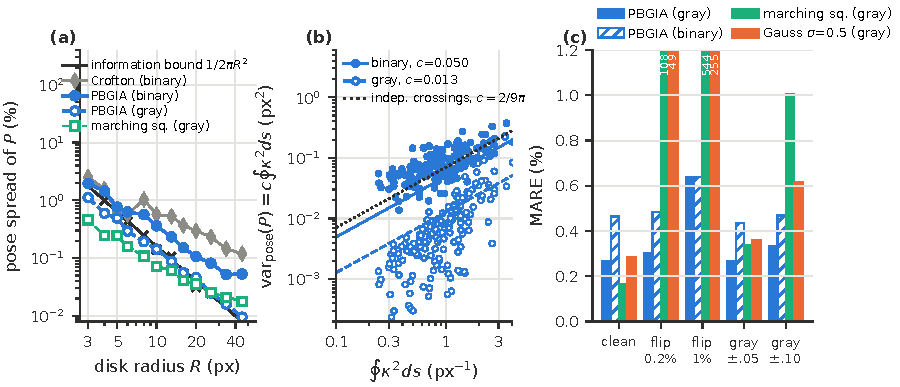
\includegraphics[width=\linewidth]{figures/FigA4_floor_gray.pdf}
\caption{\textbf{The residual error of the binary readout is rasterization, and partial-volume input lowers it.} (a) Spread of the perimeter over random poses for disks (48 poses per radius), compared with the information bound \eqref{eq:infobound} (line; crosses, sampled consistent polytopes). (b) Pose variance of every non-contact 2D test geometry (25 poses) versus $\oint\kappa^2ds$, with the fitted quantization law \eqref{eq:quantlaw}; dotted, independent grid crossings. (c) MARE of the continuous source on newly generated partial-volume test shapes, compared with the binary readout of the same images thresholded at mid level and with marching squares and Gaussian smoothing on the gray image. Flip noise inverts $g$; gray noise is additive with the stated standard deviation and clipped to $[0,1]$. Bars above the axis limit are labeled with their values.}
\label{fig:floor}
\end{figure}

\begin{figure}[h]
\centering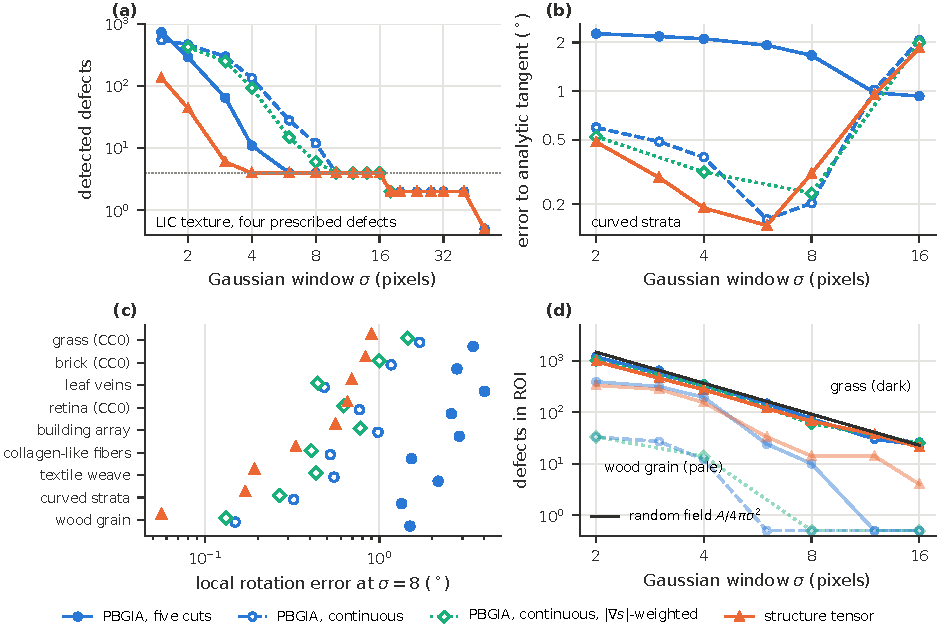
\includegraphics[width=\linewidth]{figures/FigA6_contdir.pdf}
\caption{\textbf{The continuous source improves the director on smooth textures; weighting it by $|\nabla s|$, the coarea weight of a dense threshold stack, also narrows its gap in defect isolation.} (a) Detected defects versus window for the texture with four prescribed disclinations (dotted line, four). (b) Error to the analytic tangent of the curved strata. (c) Local rotational error at $\sigma=8$ for the nine textures of Table~\ref{tab:multithresh}. (d) Defect counts in the $271^2$ region for grass (dark) and the synthetic wood grain (pale), with the random-field law. Filled circles, five-cut stack; open circles, continuous source; open diamonds, continuous source with tensors weighted by $|\nabla s|$; triangles, structure tensor.}
\label{fig:contdir}
\end{figure}

\begin{figure}[h]
\centering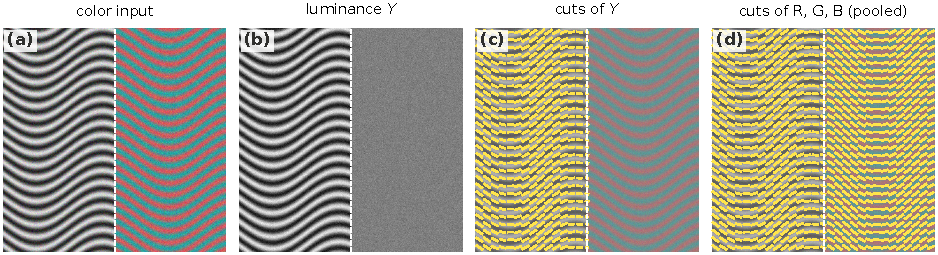
\includegraphics[width=\linewidth]{figures/FigA5_color.pdf}
\caption{\textbf{Luminance alone loses an isoluminant texture; channel-wise threshold fields recover it.} (a) Curved strata carried by luminance (left of the dashed line) and by an isoluminant chroma modulation (right), with channel noise $0.05$. (b) Luminance. (c) Director from five quantile cuts of the luminance. (d) Director from five quantile cuts of each of R, G and B, pooled as tensors. Segment length is proportional to the eigenvalue gap, normalized separately in each half; $\sigma=8$.}
\label{fig:color}
\end{figure}


\clearpage
\bibliographystyle{unsrtnat}
\bibliography{refs}

\end{document}
